%
%  Chapter:  4 - Transverse Wobbling in 135Pr
%  Modified: 2/16/2015
%  Author:   James Till Matta
%
%%%%%%%%%%%%%%%%%%%%%%%%%%%%%%%%%%%%%%%%%%%%%%%%%%%%%%%%%%

\chapter{TRANSVERSE WOBBLING IN $^{135}$Pr}
\label{chp:trw}
%As stated in chapter \ref{chp:intro} wobbling is the longest anticipated fingerprint of triaxiality. Bohr and Mottelson predicted its existence in 1969 in the first edition of the second volume of their book nuclear structure\cite{bohrMottelson2}. Despite this longstanding prediction of its existence, the first discovery of wobbling was in 2001 by \O{}deg\aa{}rd \emph{et al.} \cite{wobblingIn163Lu}. Prior to this work wobbling had only been seen in five nuclei confined to the $A\sim{}170$ region, $^{161,163,165,167}$Lu \cite{wobblingIn163Lu,wobblingIn161Lu,wobblingIn165Lu,wobblingIn167Lu} and $^{167}$Ta \cite{wobblingIn167Ta}.

%Wobbling is the harmonic vibration of a nucleus's principal axis about its angular momentum vector. In the body fixed or intrinsic frame, wobbling is the harmonic vibration of the nucleus's angular momentum vector about one of its principal axes. In the simple wobbling mode, the principal axis used as a reference is the intermediate axis. This intermediate axis has the largest moment of inertia (MOI) and absent anything else is the preferred axis of rotation. In the transverse wobbling the reference principal axis is either the short or long axes as they are the axes that a quasiparticle with primarily particle nature or hole nature will couple to respectively. This coupling forces the rotation and wobbling motion to occur about these axes, eventually though the motion will become unstable and the wobbling will collapse as the rotation realigns itself to a new vector in the plane between the intermediate axis and the original axis of rotation. The final mode, longitudinal wobbling occurs when the Coriolis force aligns the quasiparticle to the intermediate axis. As in the simple wobbling case the rotation and wobbling occurs about the intermediate axis.
Understanding of the wobbling mode in nuclei has evolved quickly over the last 15 years. Bohr and Mottelson first showed that a rotating nucleus with stable triaxially deformed could have its rotational angular momentum precess and nutate about the principal axis of a nucleus (in analogy to the classical asymmetric top) \cite{bohrMottelson2} quite some time ago. H. Schnack-Petersen \emph{et al.} suggested in 1995 that bands in $^{163,165}$Lu which are based on the $\pi{}(i_{13/2})$ configuration, occupied a triaxial superdeformed (TSD) minimum of the total routhian surface \cite{tsdLutetium}. Following this there was rash of wobbling discoveries in $^{161,163,165,167}$Lu from 2001 to 2005 \cite{wobblingIn163Lu,wobblingIn163LuTwoPhonon,wobblingIn165Lu,wobblingIn167Lu,wobblingIn161Lu}. Further searches conducted in the region on $^{171}$Ta \cite{wobbSearch171Ta}, $^{169}$Ta \cite{wobbSearch169Ta}, $^{163}$Tm \cite{wobbSearch163Tm}, $^{171,172}$Hf \cite{wobbSearch1712Hf}, and ${160,161}$Tm \cite{wobbSearch1601Tm} yielded no further wobbling bands. This left an open problem as to why wobbling was only appearing in the Lu isotopes.

A possible solution to this problem was offered up in the TAC calculations by S. Frauendorf presented in Ref. \cite{wobbSearch163Tm}. The calculations suggest that the Lu TSD minima have a low density of states, low enough that the relatively high excitation energy wobbling mode can be observed. Contrariwise, the TSD minima of other nuclei in the region had a high density of states which could produce many different TSD bands with alternate configurations at similar energies. Thus, it is not that wobbling is absent in nuclei that are not Lu isotopes, but instead, that outside of the Lu isoptopes there was a competition between wobbling and particle hole excitations that favored the latter. This result motivated a search of $^{167}$Ta for wobbling which, in 2009, yielded the first wobbling band outside the Lu isotopes.


\section{Previous Cases of Wobbling}
\label{sec:trw-prev}
One phonon wobbling was first observed in 2001 in the nucleus $^{163}$Lu by S.W. \O{}deg\aa{}rd \emph{et al.} \cite{wobblingIn163Lu}. In 2002 two phonon wobbling was observed in the same nucleus by D.R. Jensen \emph{et al.} \cite{wobblingIn163LuTwoPhonon} (partial level scheme pictured in the left panel of Fig. \ref{fig:chp4-first-wobb}). In 2003 one and two phonon wobbling was discovered in $^{165}$Lu by G. Sch\"onwa\ss{}er \emph{et al.} \cite{wobblingIn165Lu} (partial level scheme pictured in the right panel of Fig. \ref{fig:chp4-first-wobb}). Later that same year came the discovery of one phonon wobbling in $^{167}$Lu by H. Amro \emph{et al.} \cite{wobblingIn167Lu} (partial level scheme pictured in the left panel of Fig. \ref{fig:chp4-second-wobb}). 2005 was the year of the discovery of one phonon wobbling  $^{161}$Lu by P. Bringel \emph{et al.} \cite{wobblingIn161Lu} (partial level scheme pictured in the right panel of Fig. \ref{fig:chp4-second-wobb}). The last of the wobblers known prior to this work, $^{167}$Ta, was discovered in 2009 by D.J. Hartley \emph{et al.} \cite{wobblingIn167Ta} (partial level scheme pictured in Fig. \ref{fig:chp4-last-wobb}). 

\begin{figure}[ht!]
\centerline{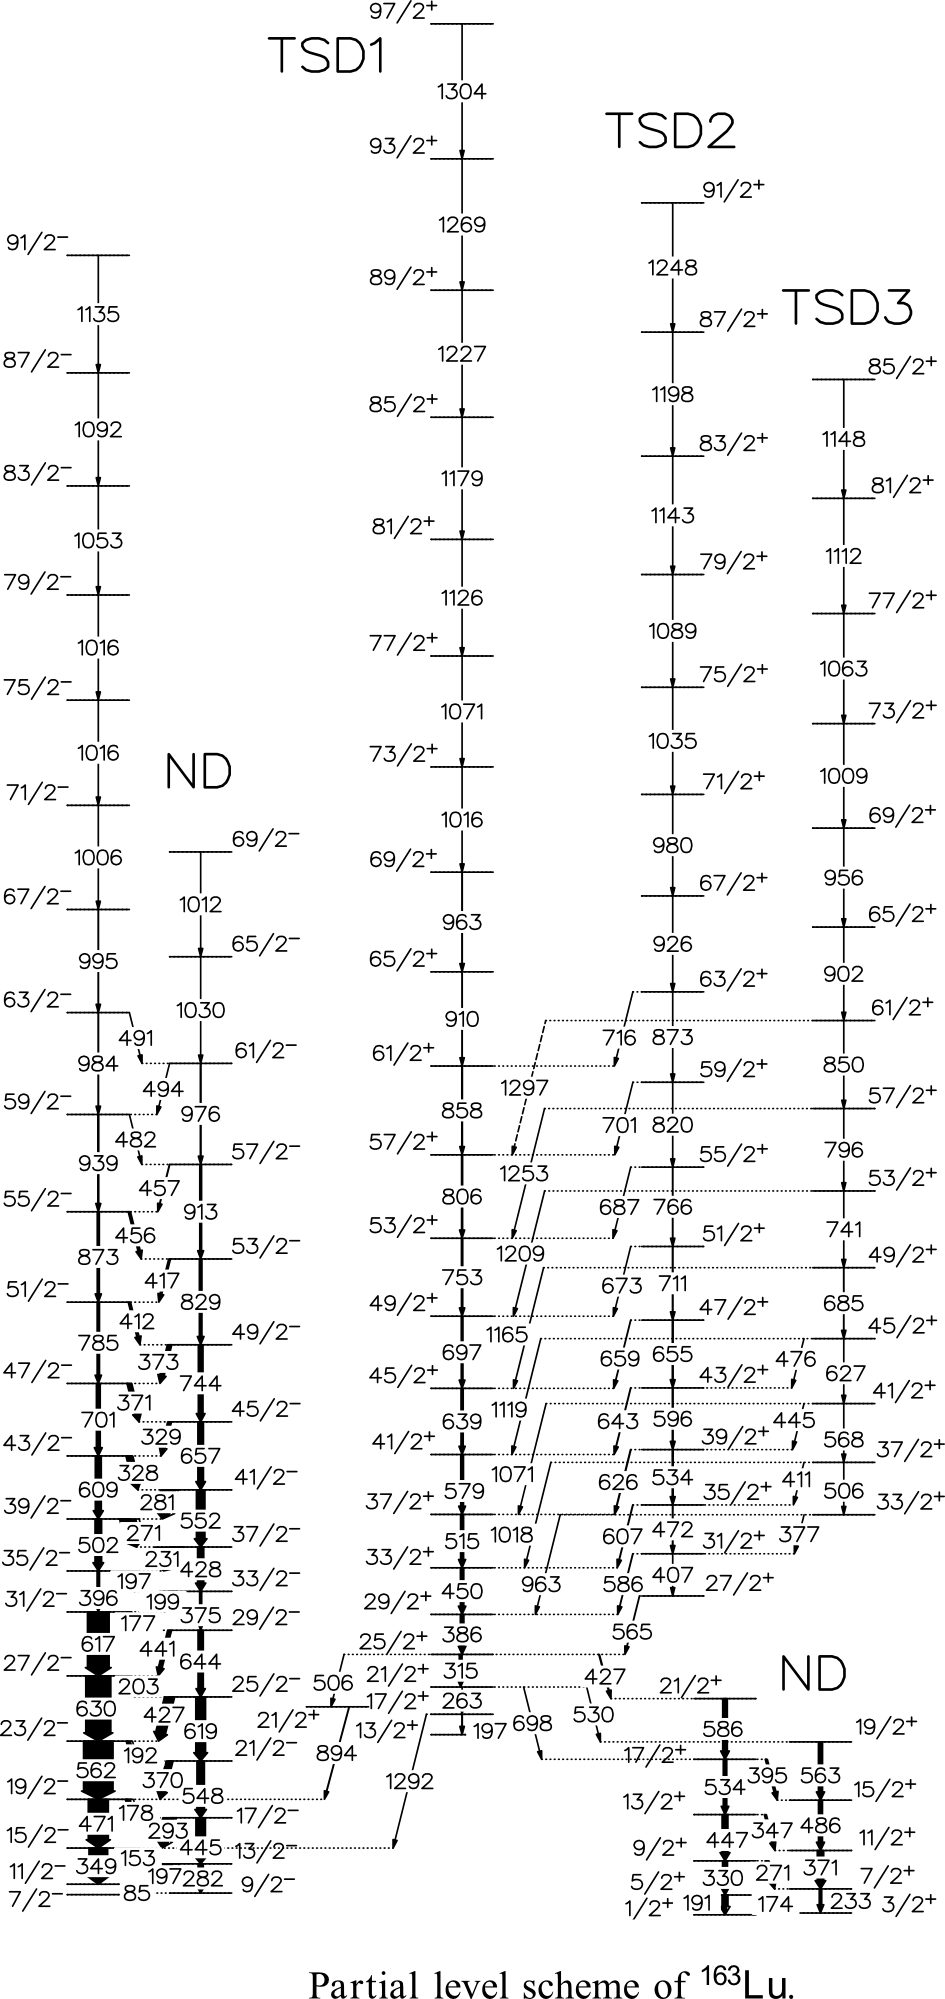
\includegraphics[width=0.4\textwidth]{./img/c4/163Lu_scheme.png}\hspace{0.1\textwidth}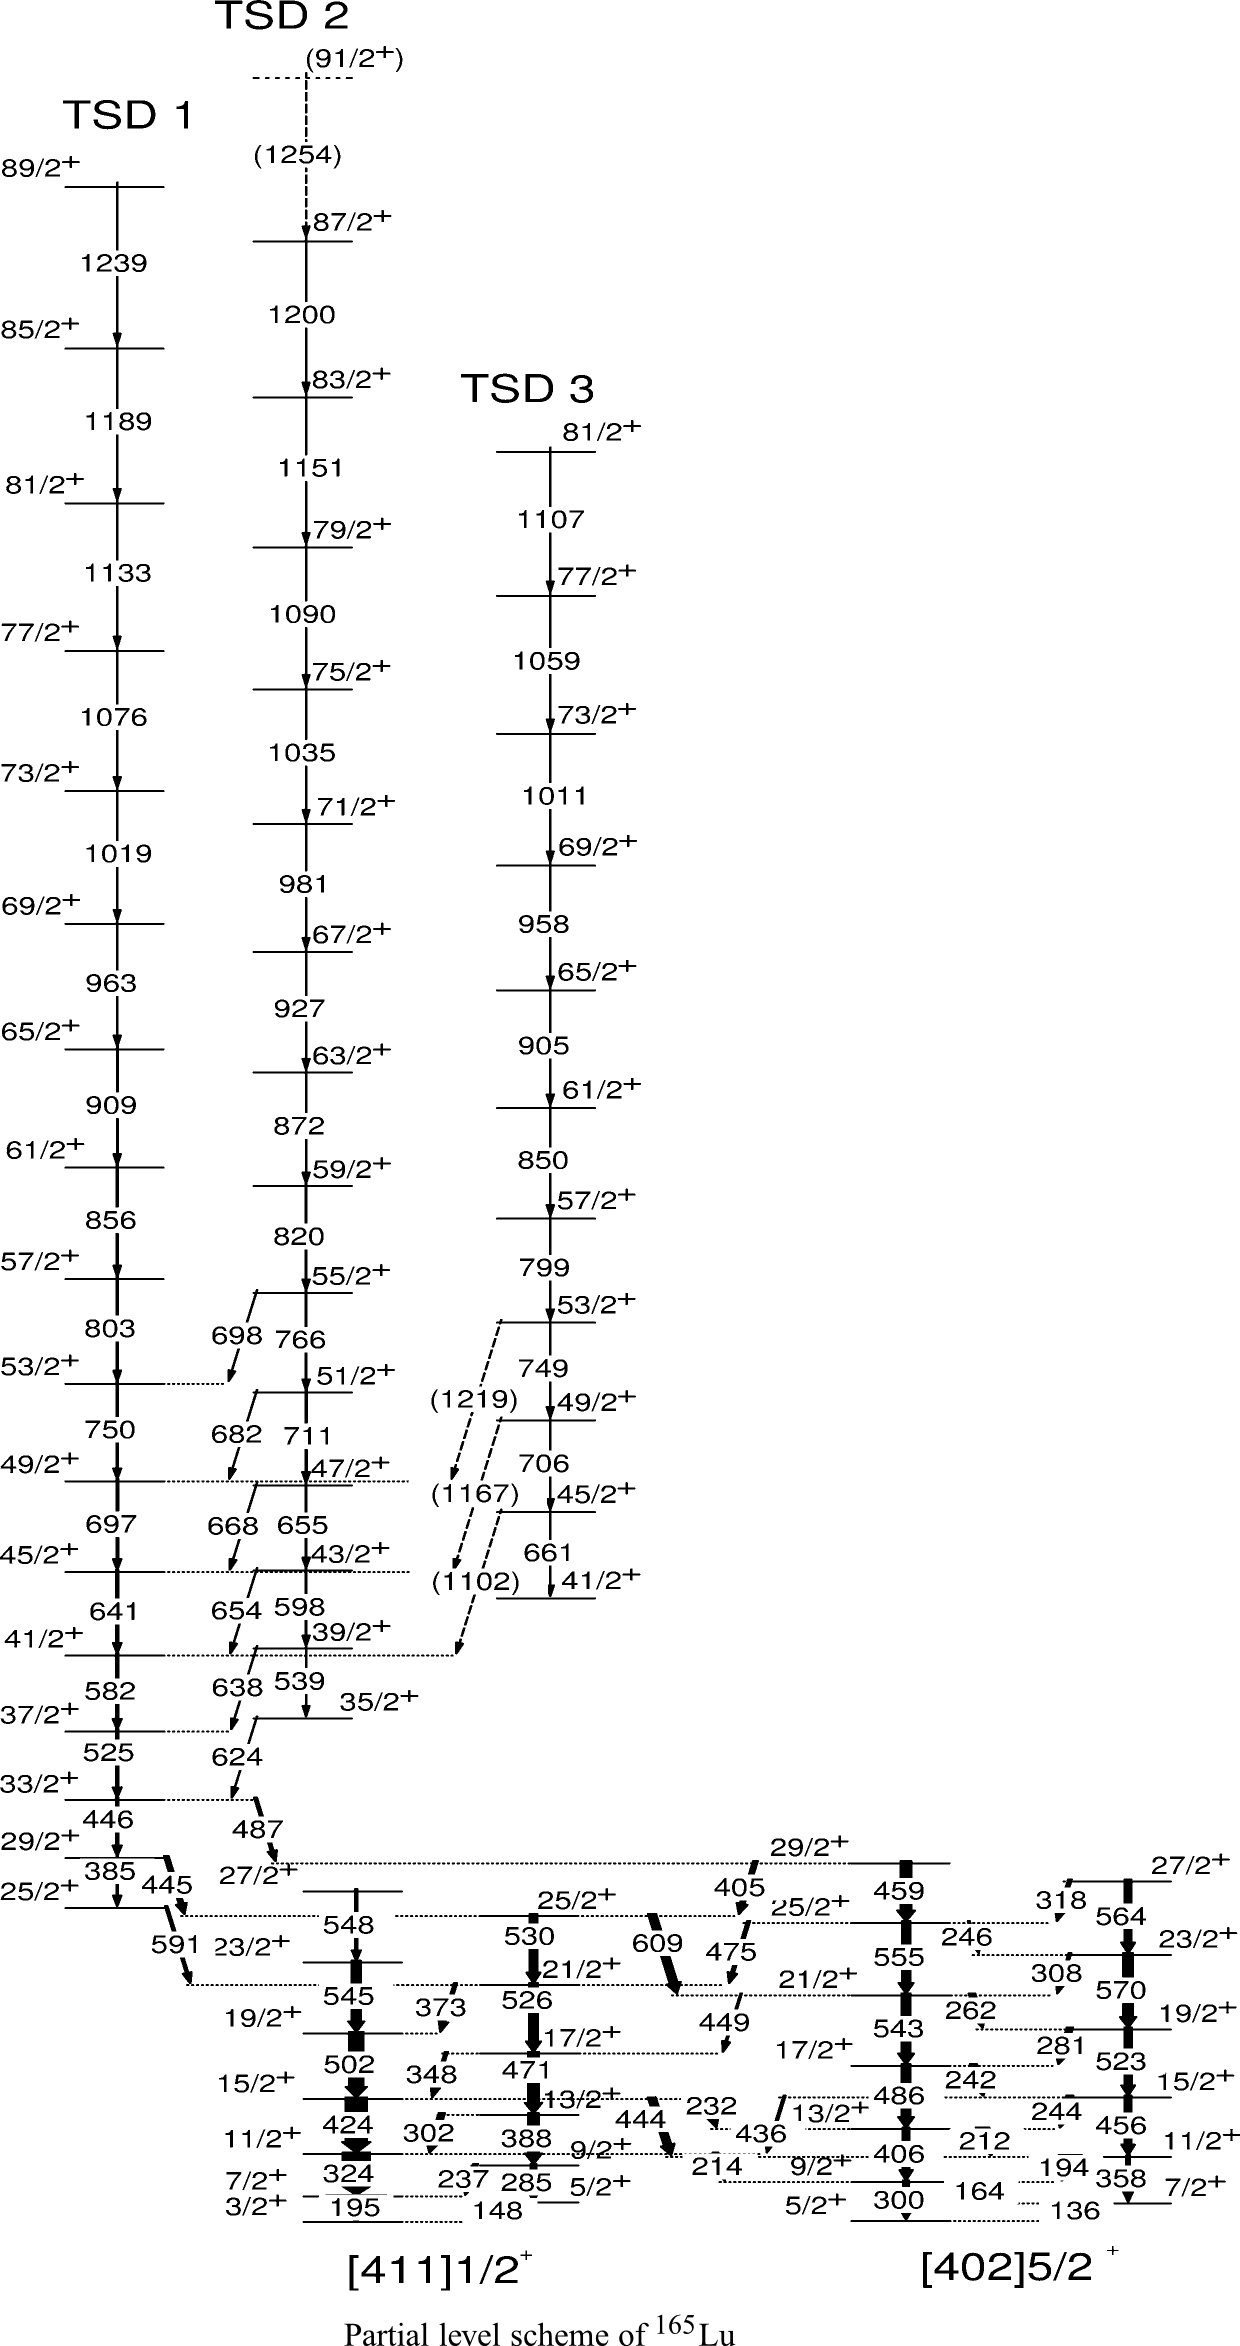
\includegraphics[width=0.4\textwidth]{./img/c4/165Lu_scheme.png}}
	\caption{Partial level schemes of $^{163}$Lu (left) and $^{165}$Lu (right). Figures adapted from Ref. \cite{wobblingIn163LuTwoPhonon} and Ref. \cite{wobblingIn165Lu} respectively. In $^{163}$Lu the $n_w=0,1,2$ bands are labeled TSD1, TSD2, and TSD3 respectively. In $^{165}$Lu the $n_w=0,1,2$ bands are labeled TSD1, TSD2, and TSD3 respectively.\label{fig:chp4-first-wobb}}
\end{figure}

\begin{figure}[ht!]
\centerline{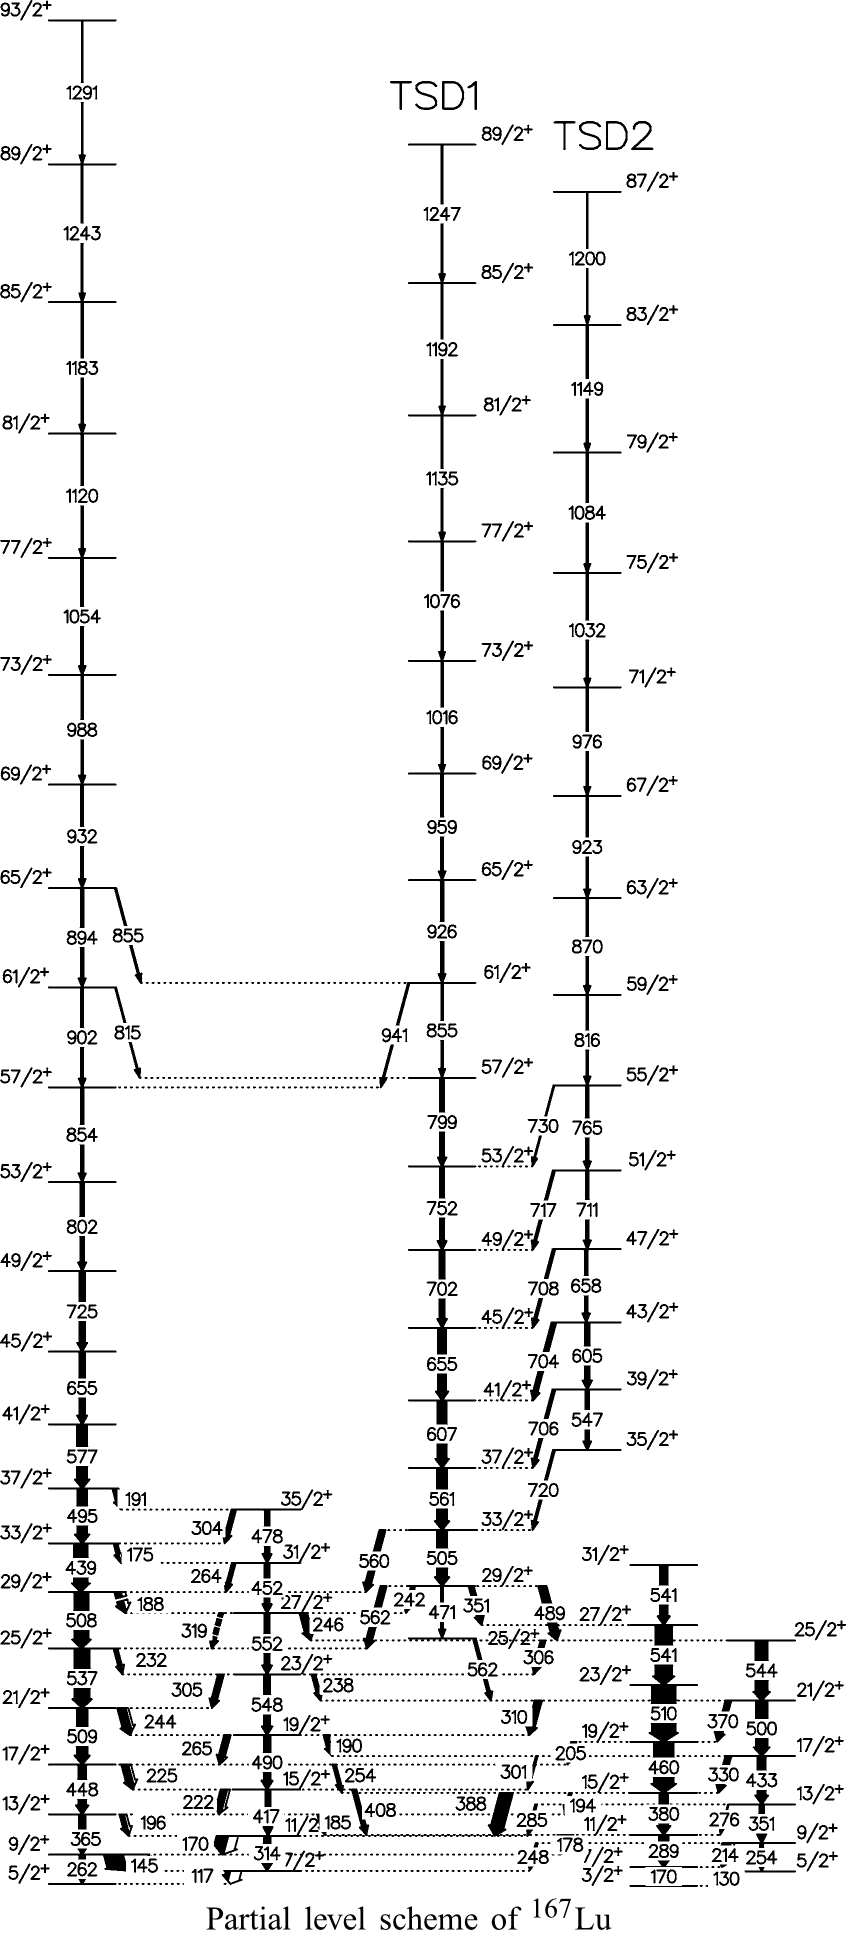
\includegraphics[width=0.4\textwidth]{./img/c4/167Lu_scheme.png}\hspace{0.1\textwidth}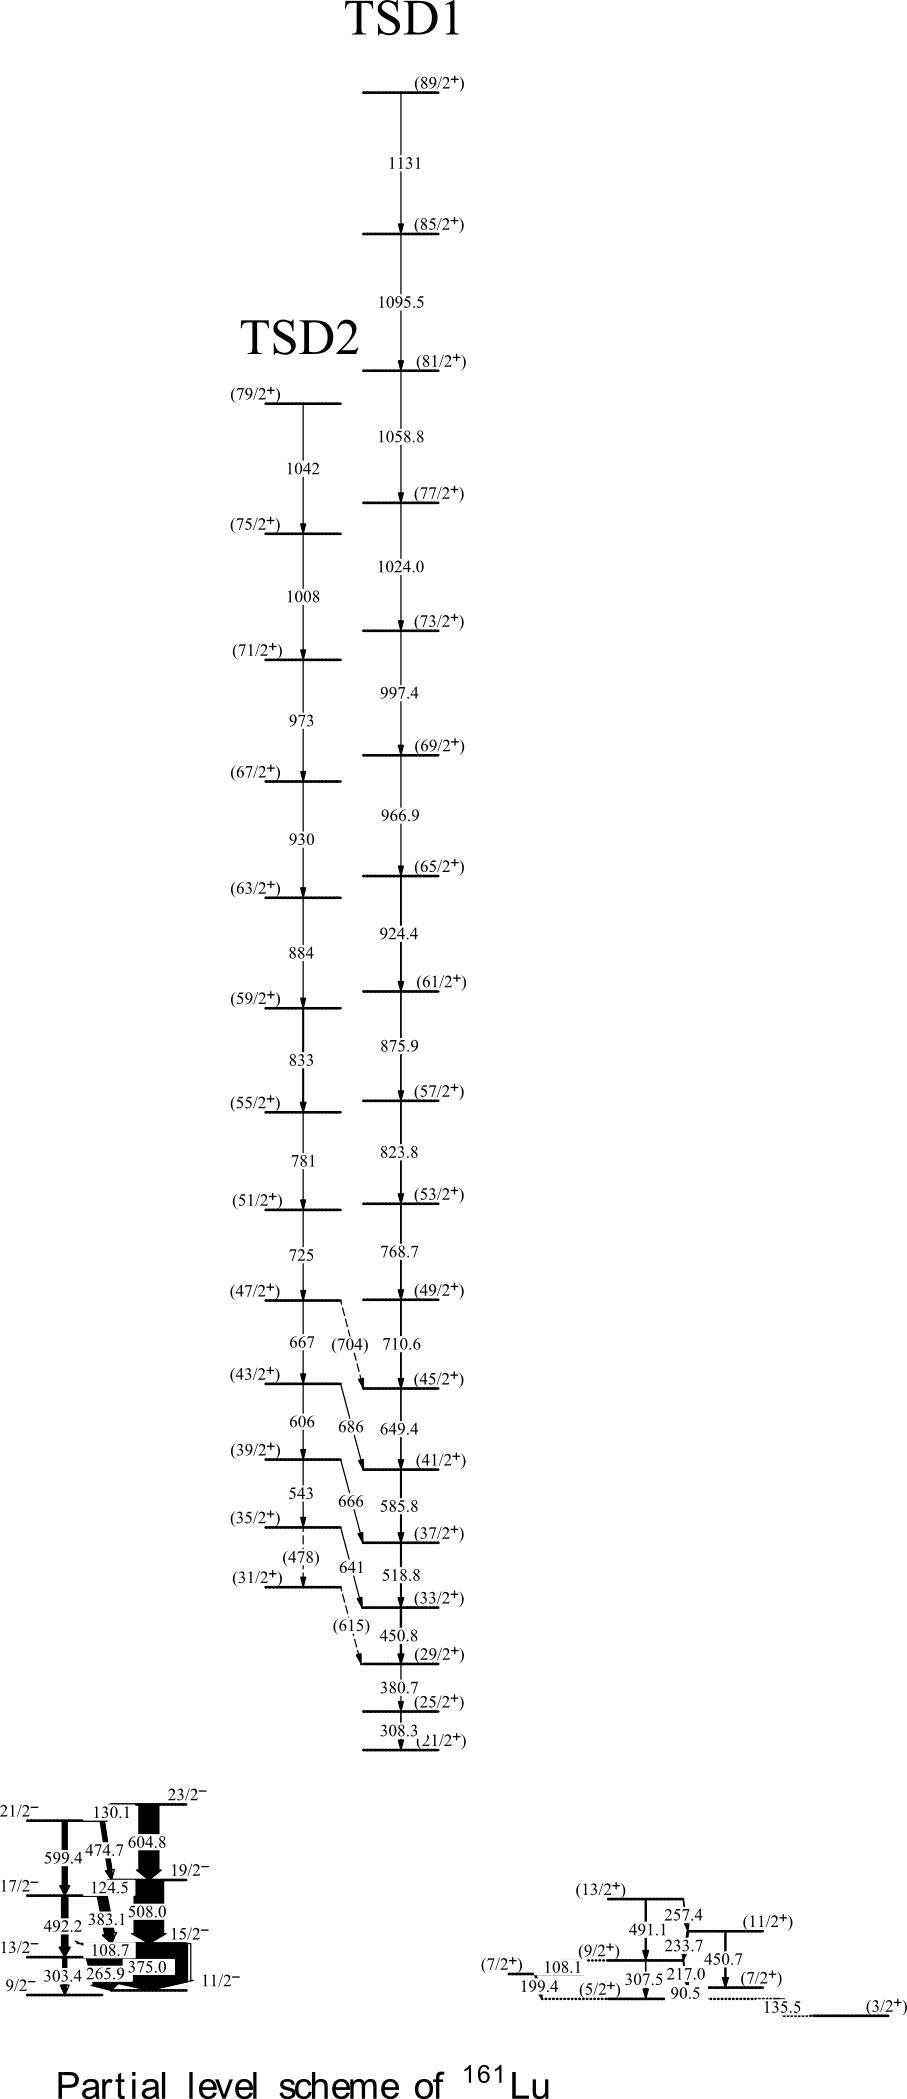
\includegraphics[width=0.4\textwidth]{./img/c4/161Lu_scheme.png}}
	\caption{Partial level schemes of $^{167}$Lu (left) and $^{161}$Lu (right). Figures adapted from Ref. \cite{wobblingIn167Lu} and Ref. \cite{wobblingIn161Lu} respectively. In $^{167}$Lu the $n_w=0,1$ bands are labeled TSD1 and TSD2 respectively. In $^{161}$Lu the $n_w=0,1$ bands are labeled TSD1 and TSD2 respectively.\label{fig:chp4-second-wobb}}
\end{figure}

\begin{figure}[ht!]
\centerline{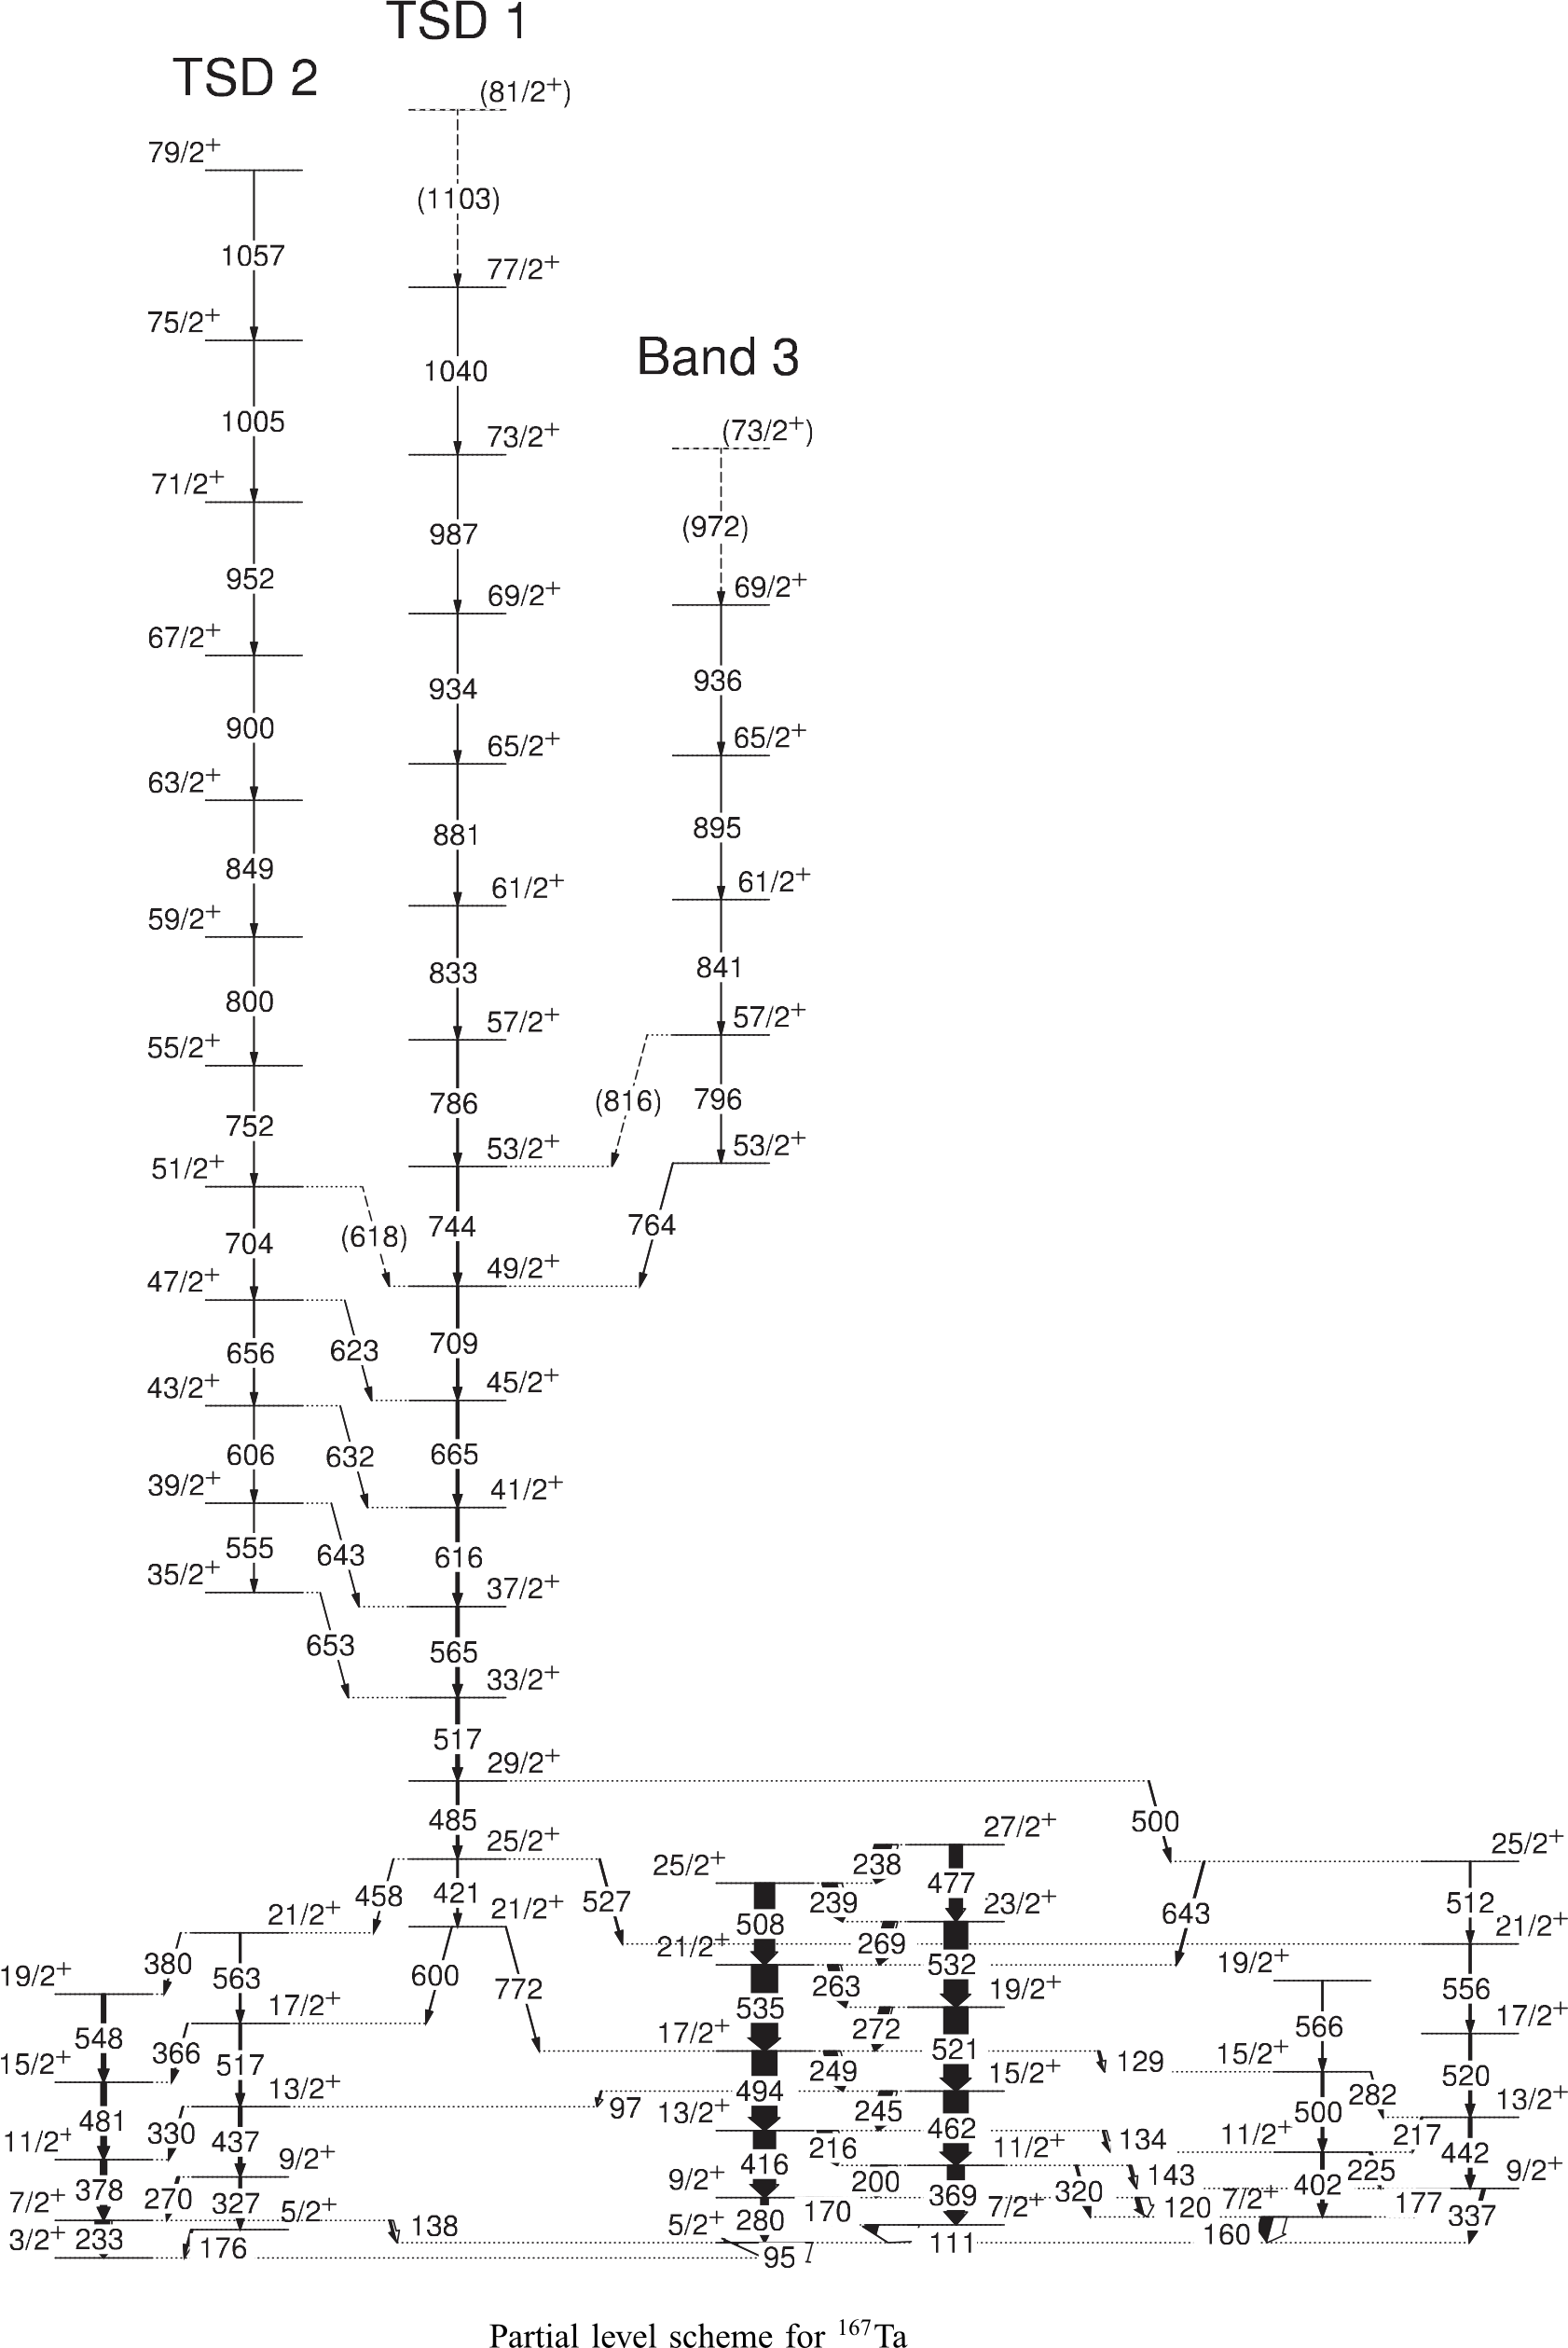
\includegraphics[width=0.6\textwidth]{./img/c4/167Ta_scheme.png}}
	\caption{Partial level scheme of $^{167}$Ta. Figure adapted from Ref. \cite{wobblingIn167Ta}. The $n_w=0,1$ bands are labeled TSD1 and TSD2 respectively.\label{fig:chp4-last-wobb}}
\end{figure}

Following the discovery of the first wobbling structure, calculations using the QTR model were used to describe the wobbling mode \cite{oldQTRWobblingTheory1,oldQTRWobblingTheory2,oldQTRWobblingTheory3,oldQTRWobblingTheory4}. Later, microscopic random phase approximation (RPA) calculations \cite{wobblingRPAMatsuzaki,wobblingRPAMatsuzaki2,wobblingRPAOi,wobblingRPAShimizu,wobblingRPAshoji} were used as well. Both theories do well in reproducing the large $B(E2)_{out}/B(E2)_{in}$ interband to intraband ratios seen in experiment. However, the QTR model, using the assumptions that the odd quasiparticle aligns with the intermediate axis \cite{oldQTRWobblingTheory1,oldQTRWobblingTheory2,oldQTRWobblingTheory3,oldQTRWobblingTheory4}, failing to reproduce the experimentally observed decrease in the wobbling energy (see Fig. \ref{fig:chp4-old-wobb-freq}) which is defined by:
\begin{equation}
\label{eqn:chp4-wobb-freq}
\Delta{}E=\hbar\omega_w(I)=E(I,n_w=1)-(E(I-1,n=0)+E(I+1,n_w=0))/2
\end{equation}
In constrast the microscopic RPA calculations were able to reproduce the observed decrease in wobbling energy.
\begin{figure}[ht!]
\centerline{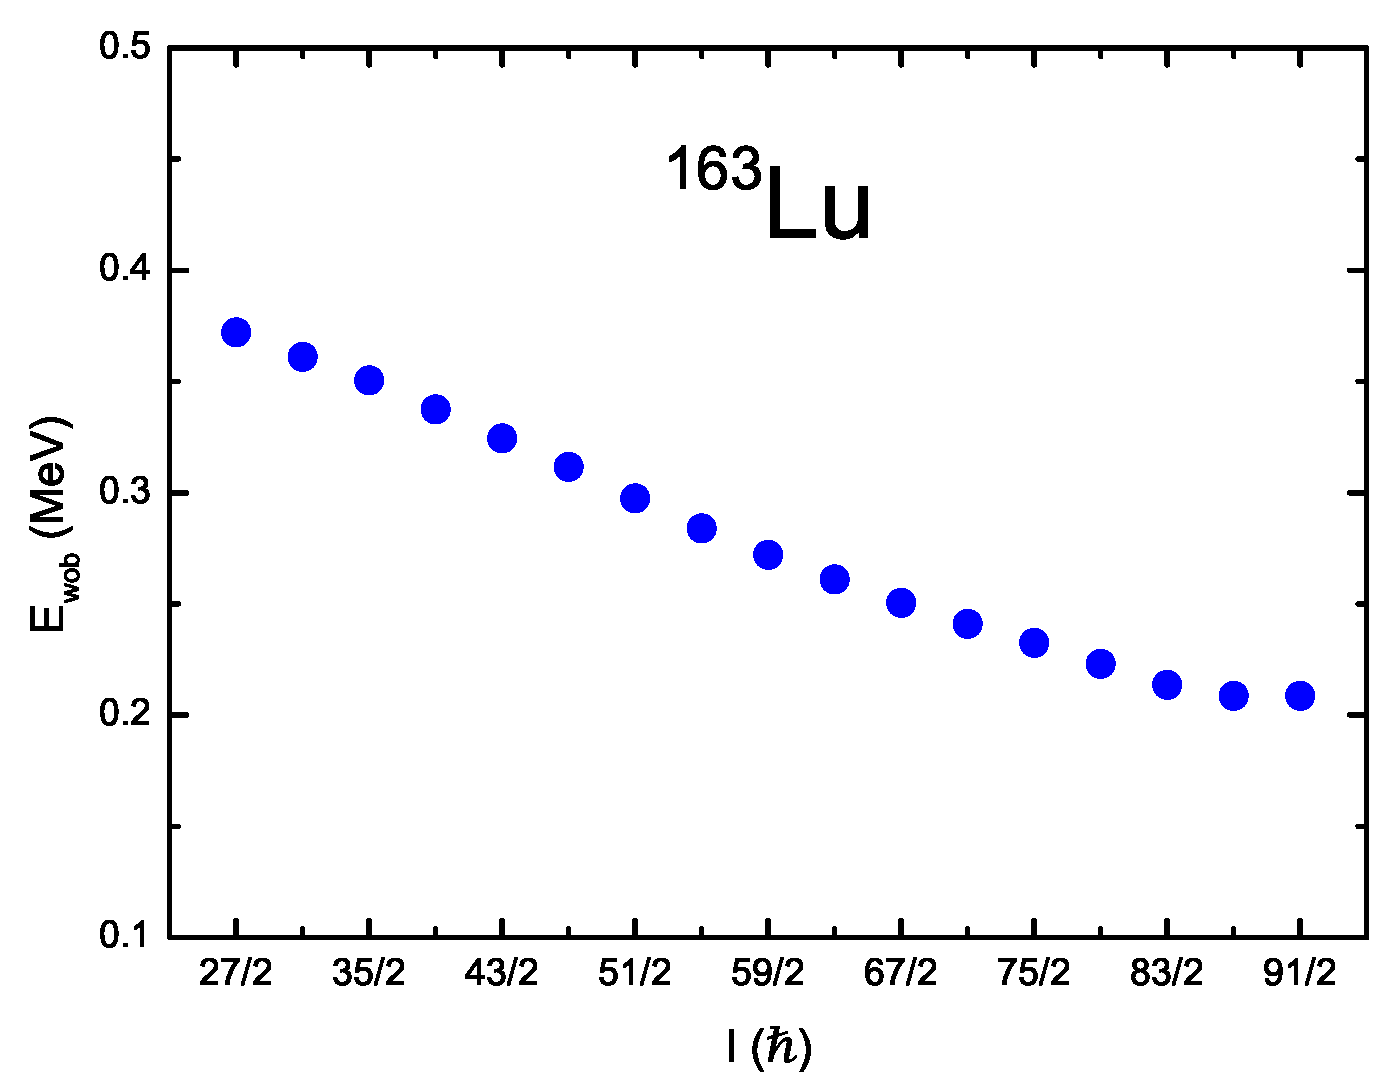
\includegraphics[height=0.25\textheight]{./img/c4/163Lu_plot.eps}\hspace{0.1\textwidth}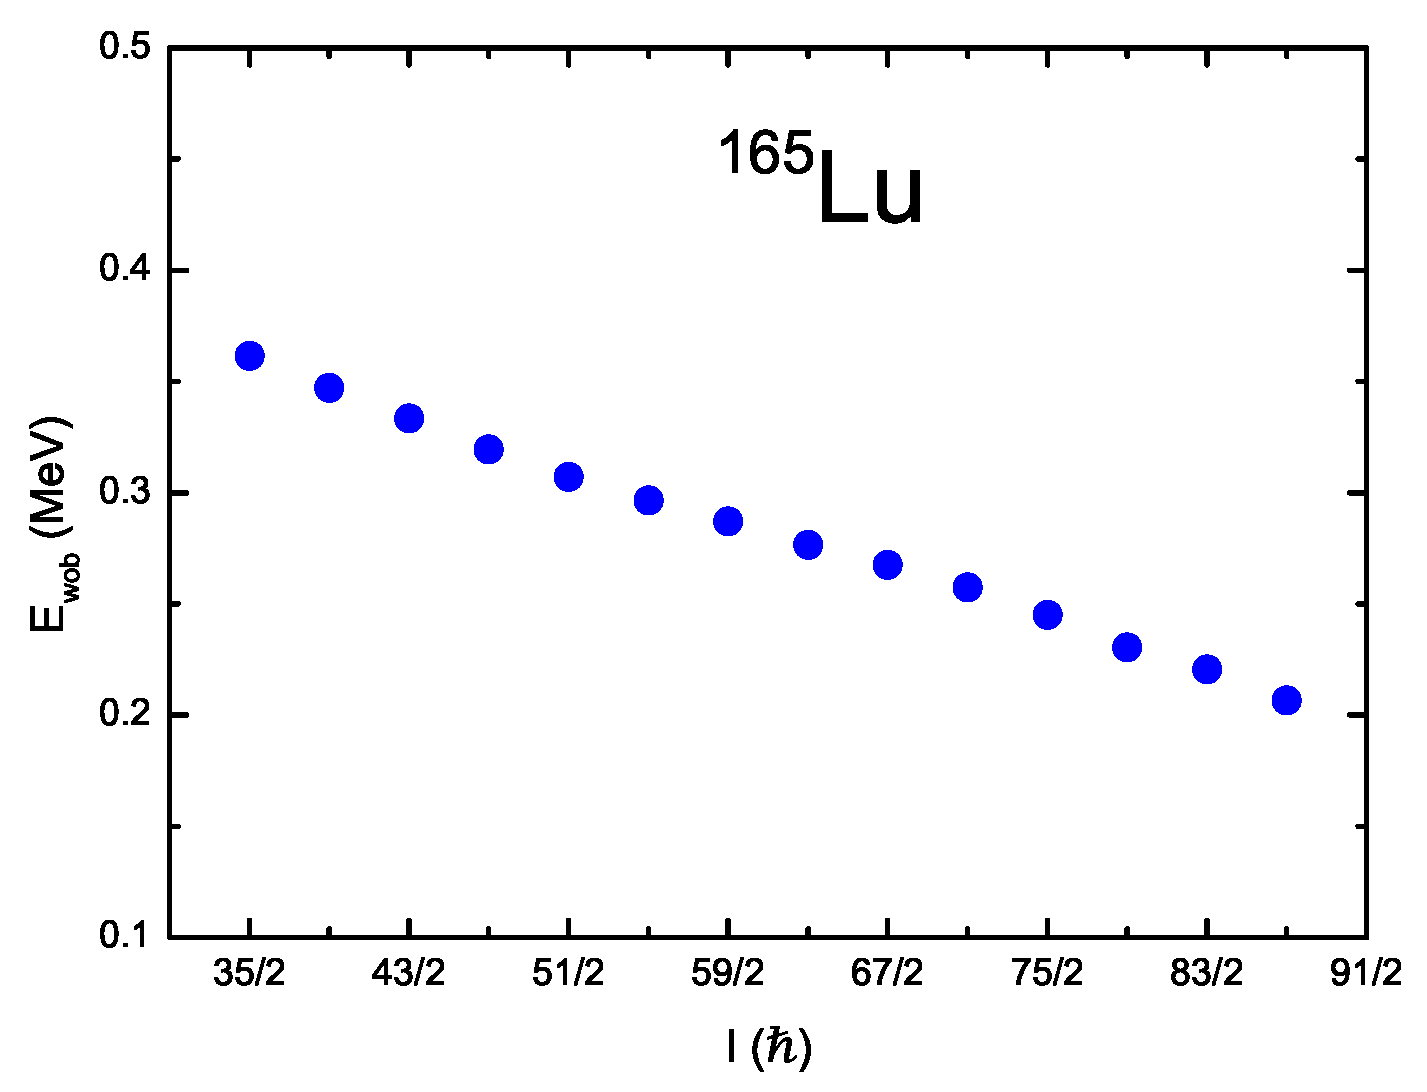
\includegraphics[height=0.25\textheight]{./img/c4/165Lu_plot.eps}}
\centerline{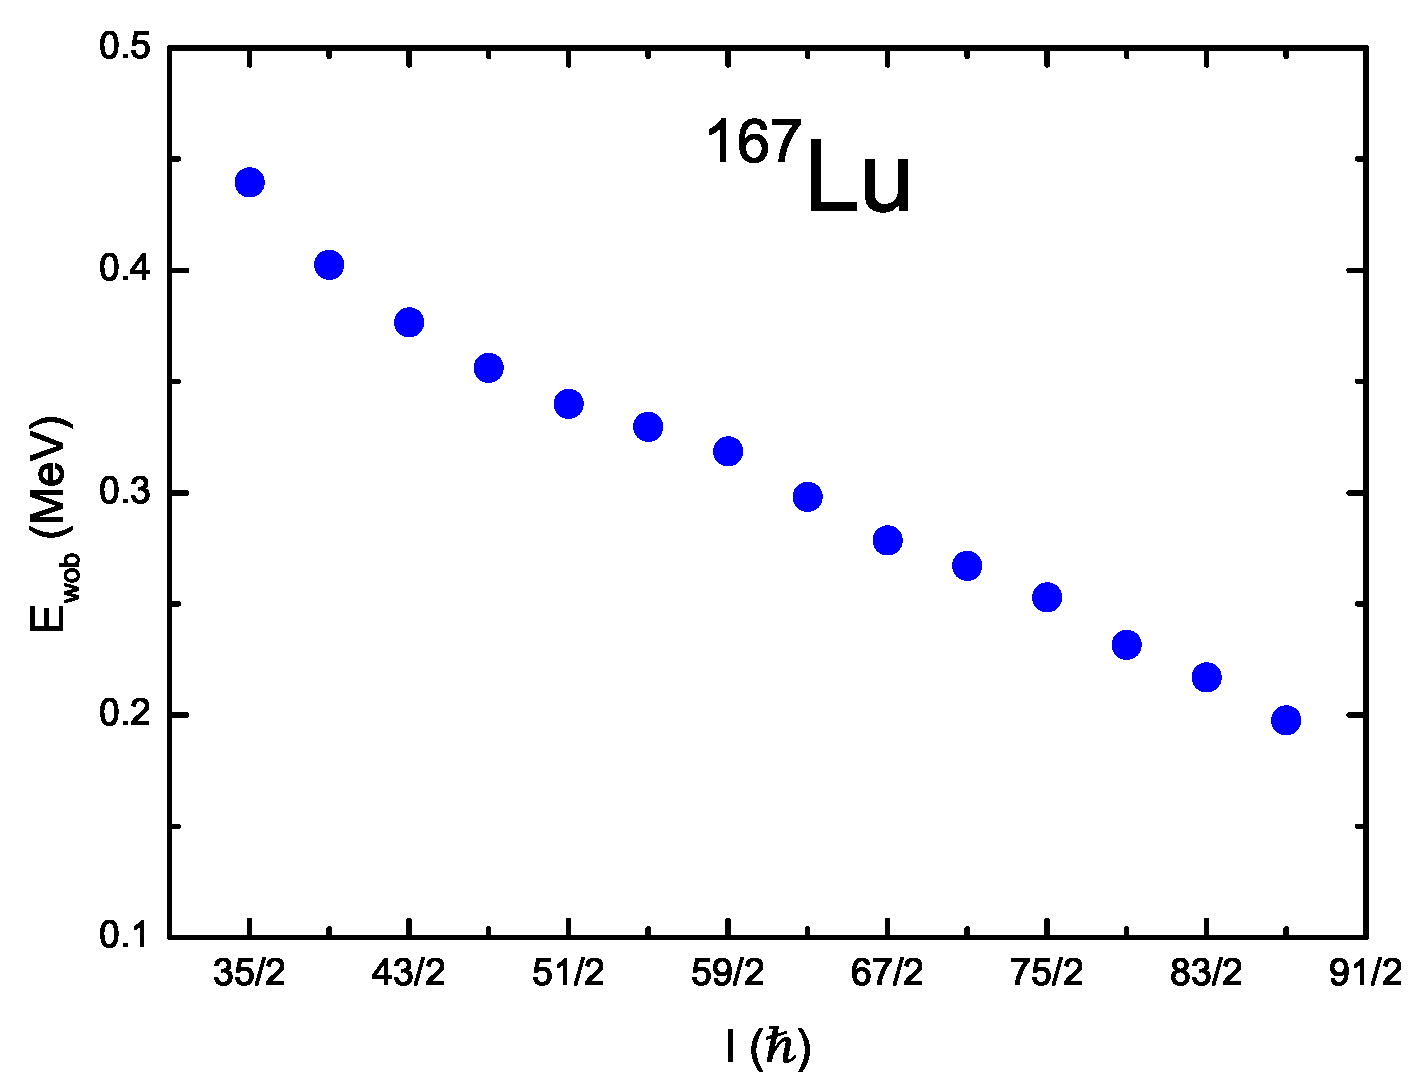
\includegraphics[height=0.25\textheight]{./img/c4/167Lu_plot.eps}\hspace{0.1\textwidth}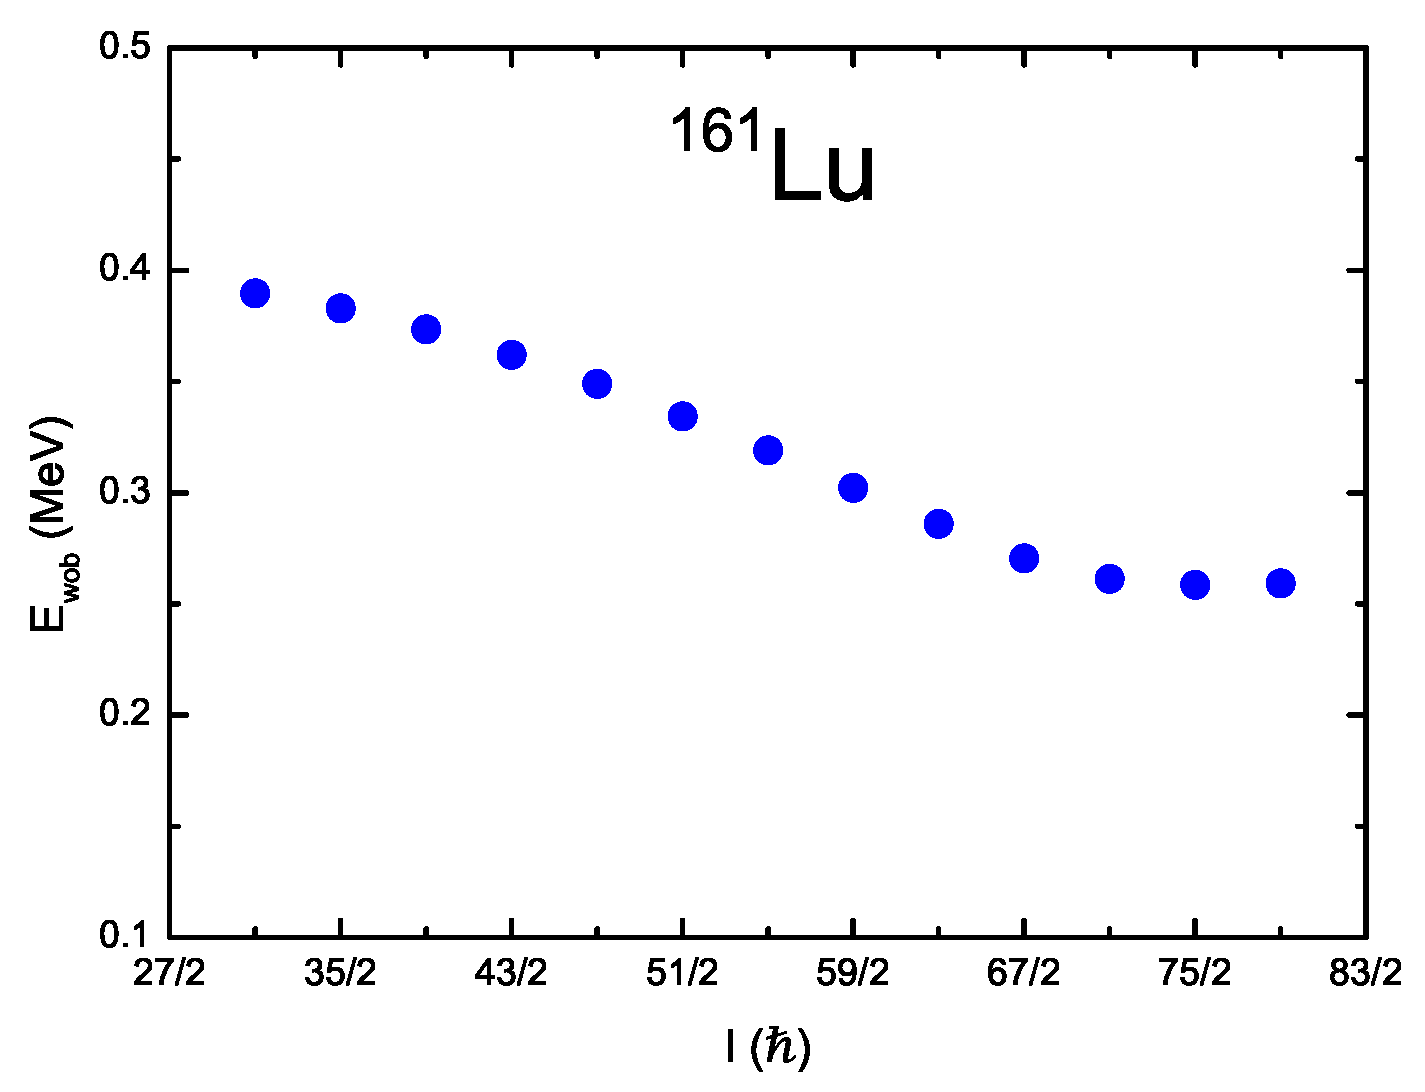
\includegraphics[height=0.25\textheight]{./img/c4/161Lu_plot.eps}}
\centerline{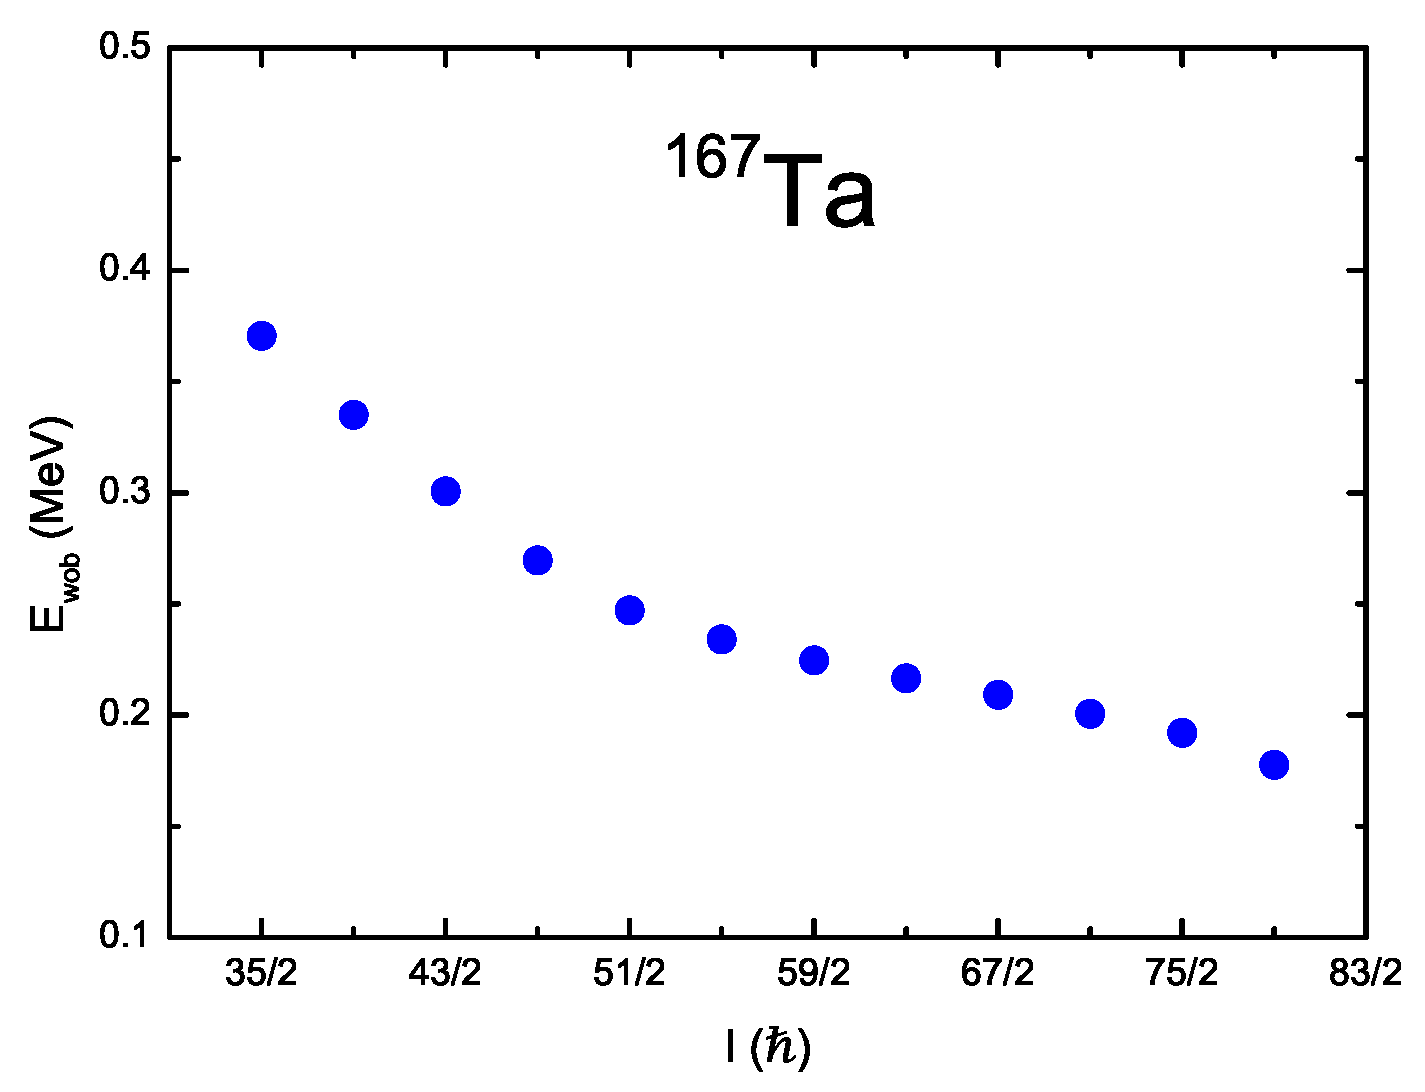
\includegraphics[height=0.25\textheight]{./img/c4/167Ta_plot.eps}}
	\caption{Wobbling frequencies of the $A\sim{}170$ wobblers. Top Left: $^{163}$Lu. Top Right: $^{165}$Lu. Middle Left: $^{167}$Lu. Middle Right: $^{161}$Lu. Bottom: $^{167}$Ta.\label{fig:chp4-old-wobb-freq}}
\end{figure}

To correct the deficiency in the QTR calculations of wobbling, S. Fraendorf and F. D\"onau introduced the concept of transverse and longitudinal wobbling \cite{frauendorfTransverseWobbling}. In this new scheme Refs. \cite{oldQTRWobblingTheory1,oldQTRWobblingTheory2,oldQTRWobblingTheory3,oldQTRWobblingTheory4} were describing longitudinal wobbling which is indeed expected to have an increasing wobbling frequency. A semi-classical analysis of transverse wobbling, which has the quasiparticle couple to an axis perpendicular to the intermediate axis, shows that the modified mode exhibits a decreasing wobbling frequency as has been seen in experimental observations of wobbling while reproducing the interband to intraband $B(E2)$ ratios.


\section{Triaxiality in the A$\sim{}130$ Region}
\label{sec:trw-triax}
As mentioned earlier in this dissertation, the wobbling mode is signature of stable triaxial deformation. That is to say that without stable triaxial shapes the there will be no wobbling excitations. As triaxiality has been a subject of general interest to the nuclear structure community for many years this makes observation of the wobbling mode important as constitutes irrefutable evidence of triaxiality. 

Another important signature of triaxial shape is nuclear chirality. Here a particle-like quasiparticle couples to the short axis, a hole like quasi-particle couples to the long axis, and the triaxial rotor core rotates about the intermediate axis. In this configuration the total angular momentum points away from any of the principal planes of the nucleus and its the three components form a screw with respect to it \cite{frauendorfChirality}. When this configuration is present, the time-reversal symmetry of the wave functions is broken and two nearly degenerate $\Delta{}I=1$ bands with similar electromagnetic properties emerge. Without triaxiality this situation cannot arise and therefore observation of nuclear chirality again gives proof of a stable triaxial shape.

Predictions made by M\"oller \emph{et al.} in Ref. \cite{groundStateTriax} show that the region around $Z=60$ and $N=76$ has triaxial shapes at low to moderate spin. This prevalence of triaxial shapes in this region is confirmed by the numerous observations of chirality \cite{chiralityIn134Pr,chiralityA130Region,chiralityA130Region2,chiralityUpperA130Region,chirality136Pm,chiralityMore135Nd,chiralityMulti133Cs,chiralityMore135Nd}. Additionally, a more exotic and stable chirality was identified in \cite{chiralityMore135Nd} and confirmed via lifetime measurement to extract the $B(M1)$ and $B(E2)$ values of the partner bands to ensure that they are the same \cite{chiralityIn135Nd}. In fact, in this observation a transition from more usual chiral vibration (where the angular momentum vector oscillates in a plane perpendicular to the axes the quasiparticles are coupled to) to static chirality where this oscillation slows to nearly stationary resulting in the bands becoming quite close to degenerate.

\section{Level Scheme of $^{135}$Pr}
\label{sec:trw-lvl-scheme}
Data from the Gammasphere experiment, described in \ref{sec:exp-pr-details}, were sorted into symmetrized cubes (E$_{\gamma{}}$-E$_{\gamma{}}$-E$_{\gamma{}}$) and hypercubes (E$_{\gamma{}}$-E$_{\gamma{}}$-E$_{\gamma{}}$-E$_{\gamma{}}$) using the RADWARE suite of codes \cite{radware}. Background subtracted gated spectra were obtained using the RADWARE suite coupled with the background subtraction algorithm of Ref. \cite{symBGSub}. The smooth backgrounds used for this algorithm are shown in Fig. \ref{fig:chp4-bg-specs}. Coincidence relations from this data were used to reconstruct the level scheme.
\begin{figure}[bh!]
\centerline{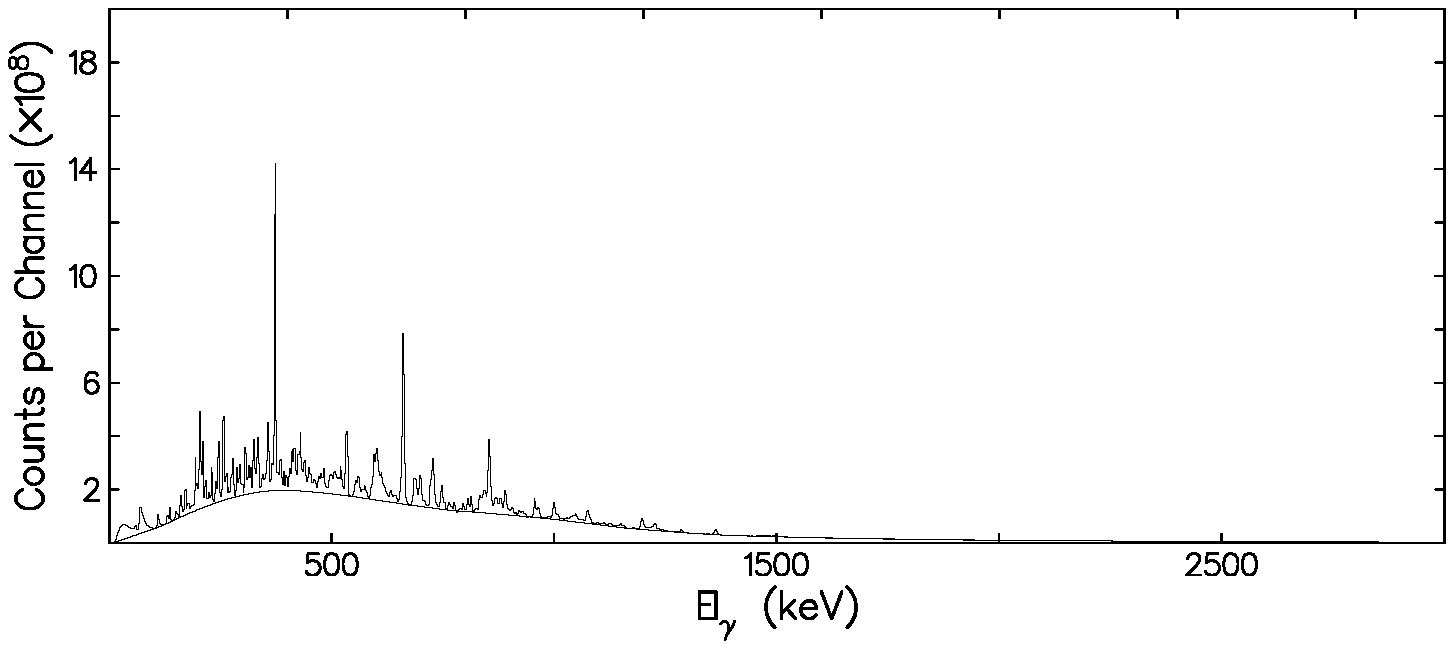
\includegraphics[width=0.45\textwidth]{./img/c4/trips_bg.pdf}\hspace{0.09\textwidth{}}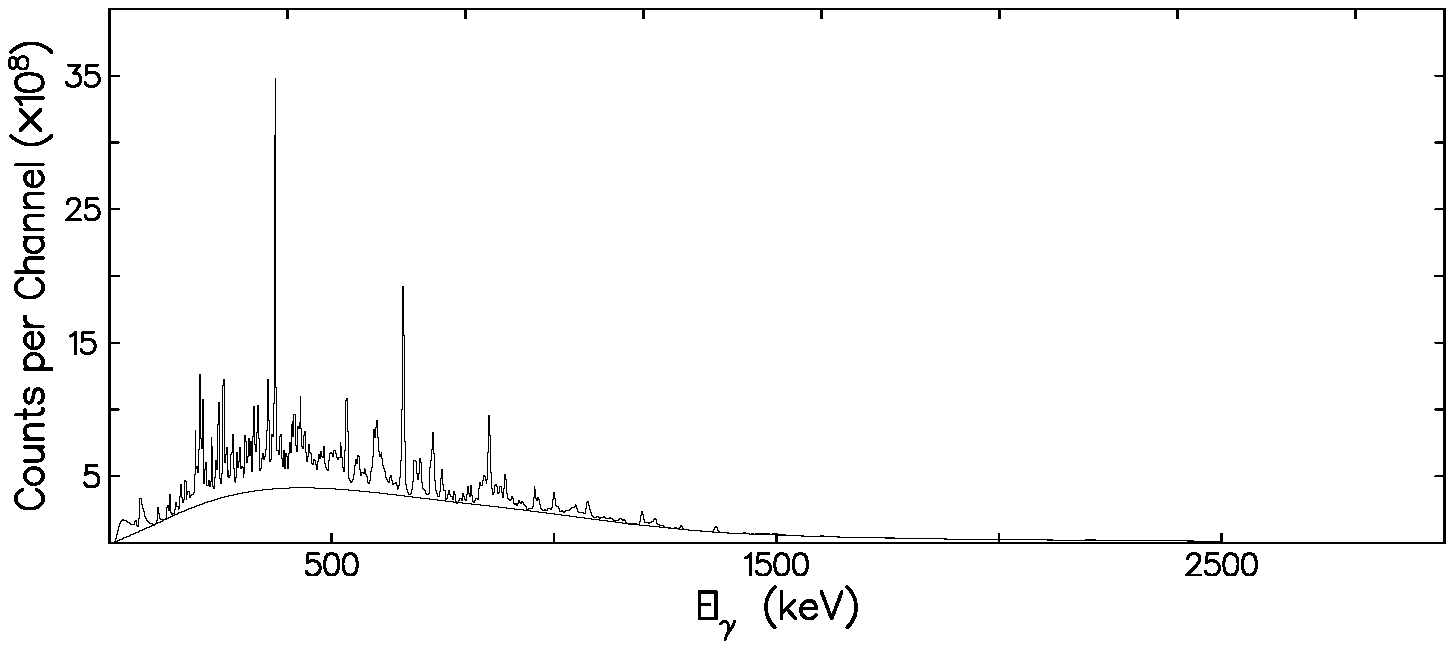
\includegraphics[width=0.45\textwidth]{./img/c4/quads_bg.pdf}}
	\caption{Left: Background spectrum for the symmetrized cube. Right: Background spectrum for the symmetrized hypercube. \label{fig:chp4-bg-specs}}
\end{figure}

\begin{figure}[ht!]
\centerline{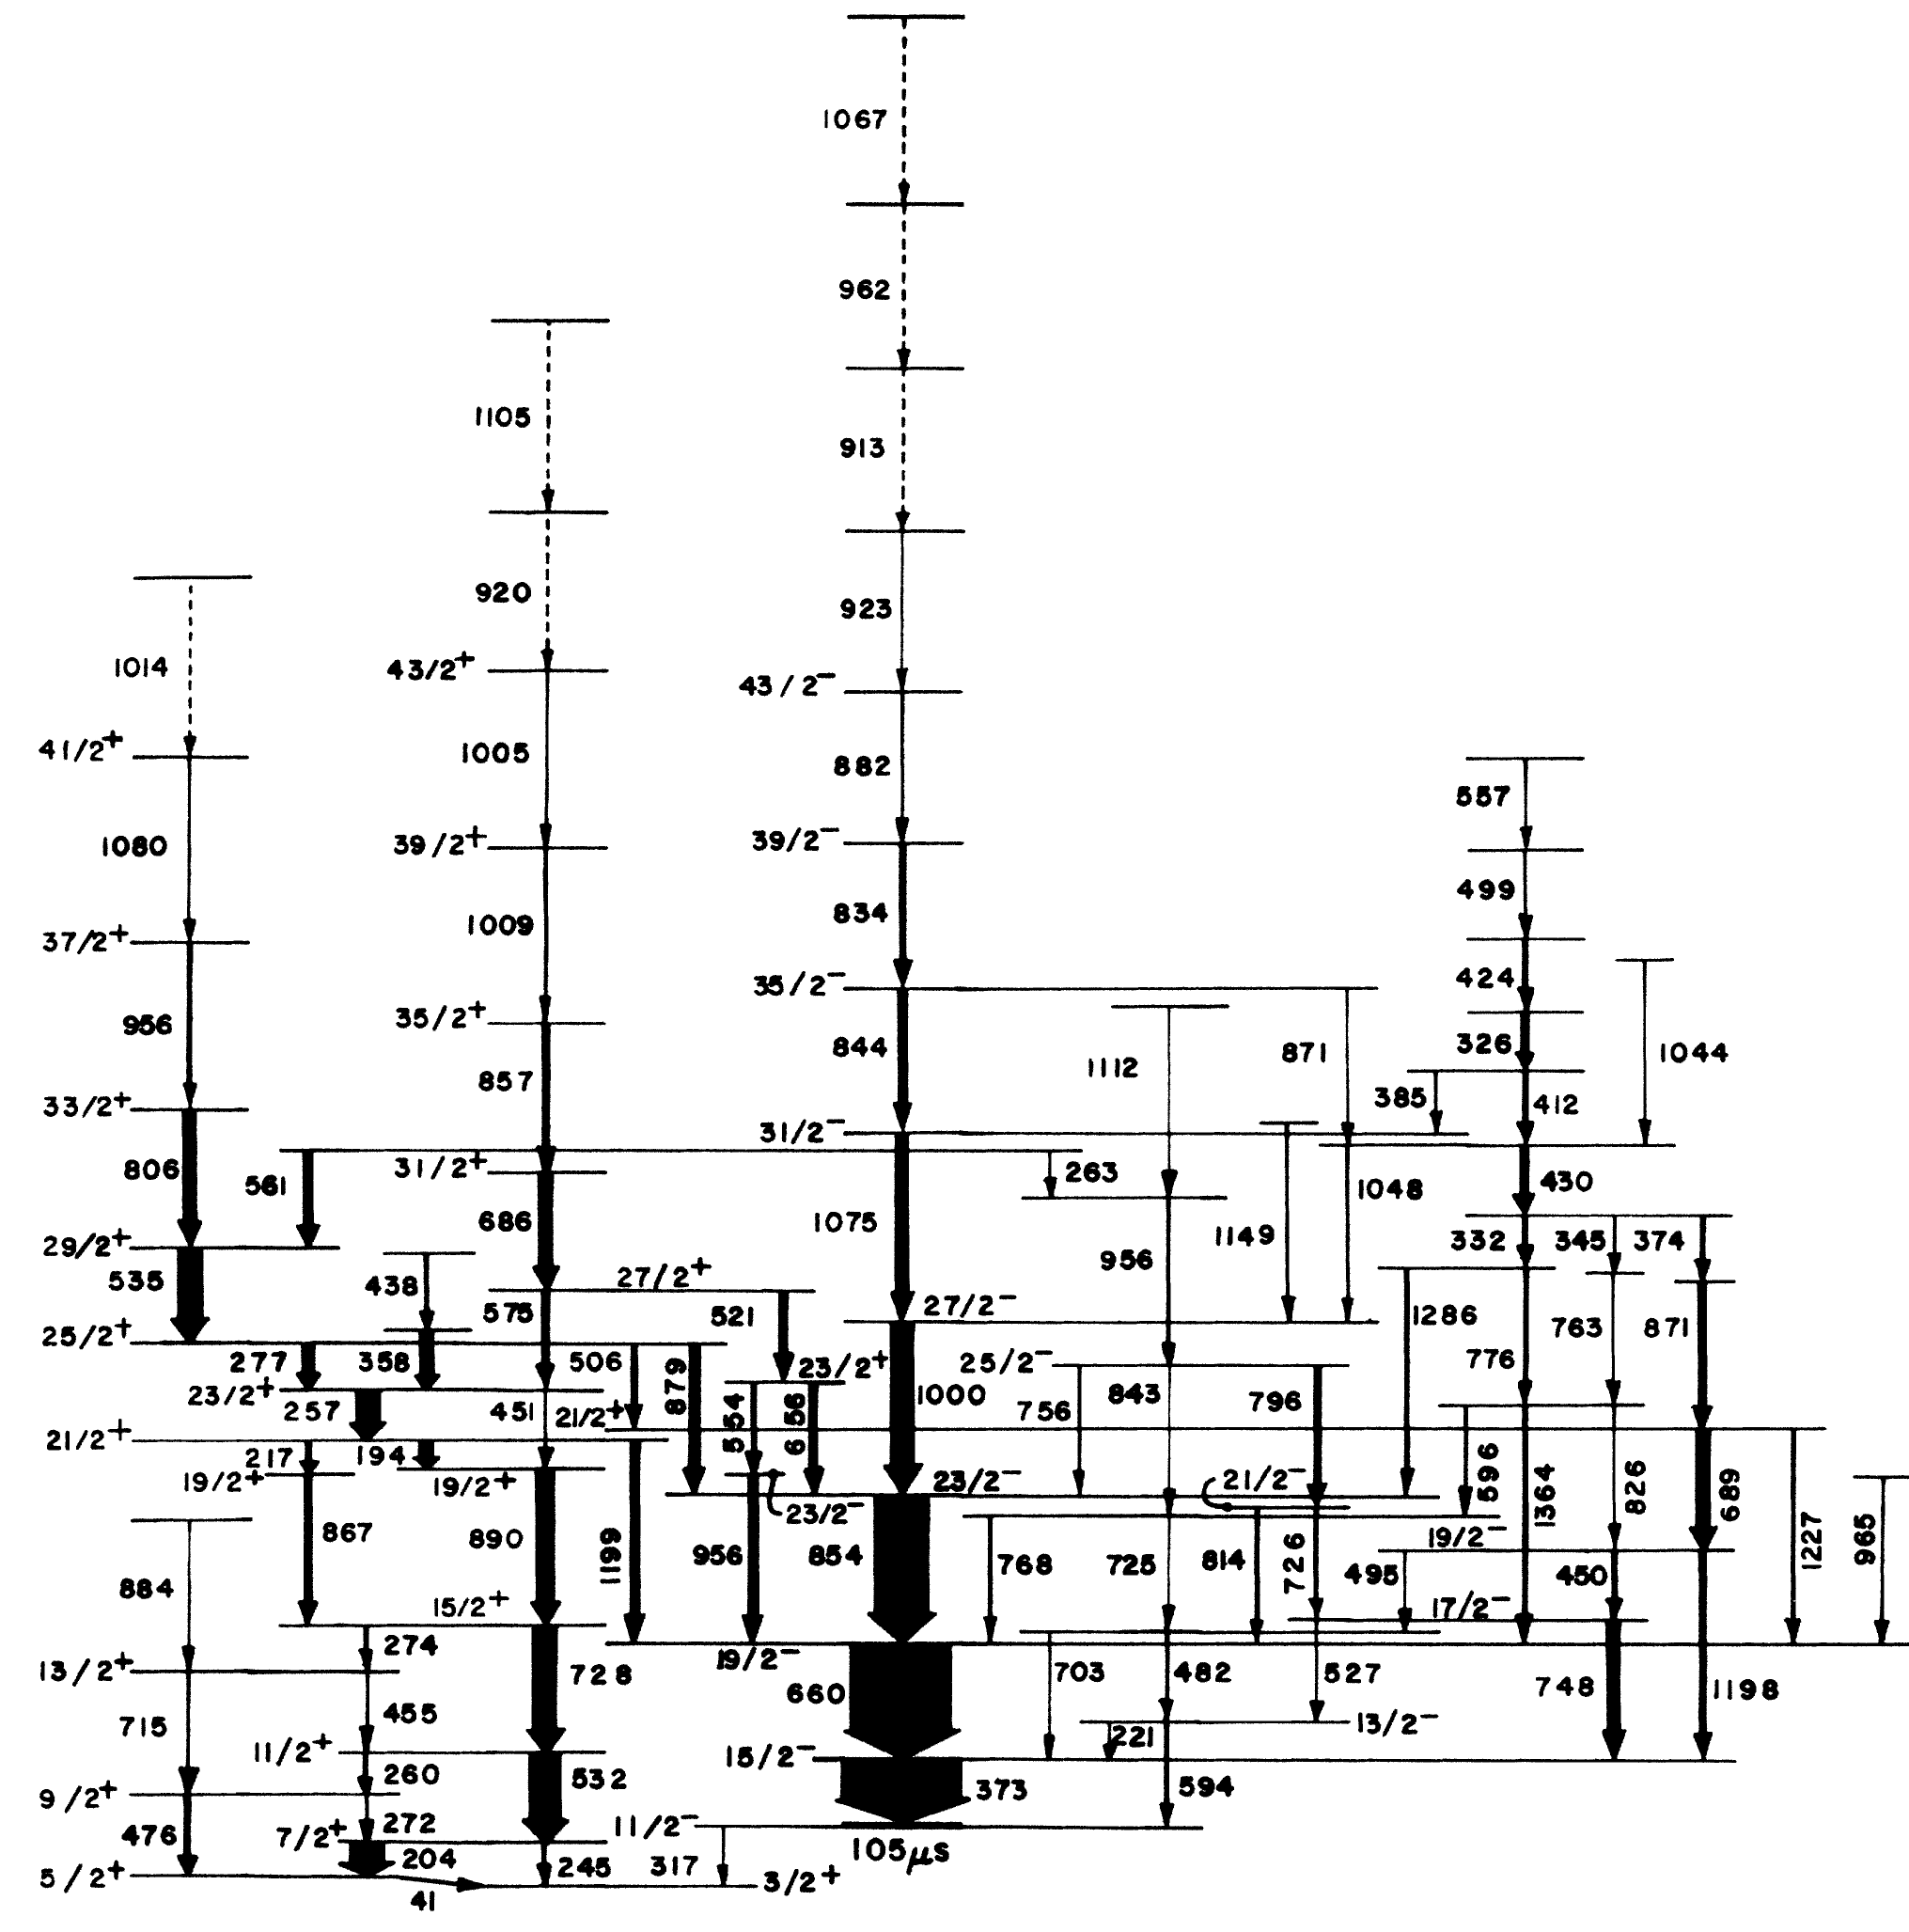
\includegraphics[width=\textwidth]{./img/c4/old_scheme.png}}
	\caption{Previous level scheme for \pr{}, from Ref. \cite{semkow135Pr}. \label{fig:chp4-semkow-lvl-schm}}
\end{figure}

\begin{figure}[hb!]
\centerline{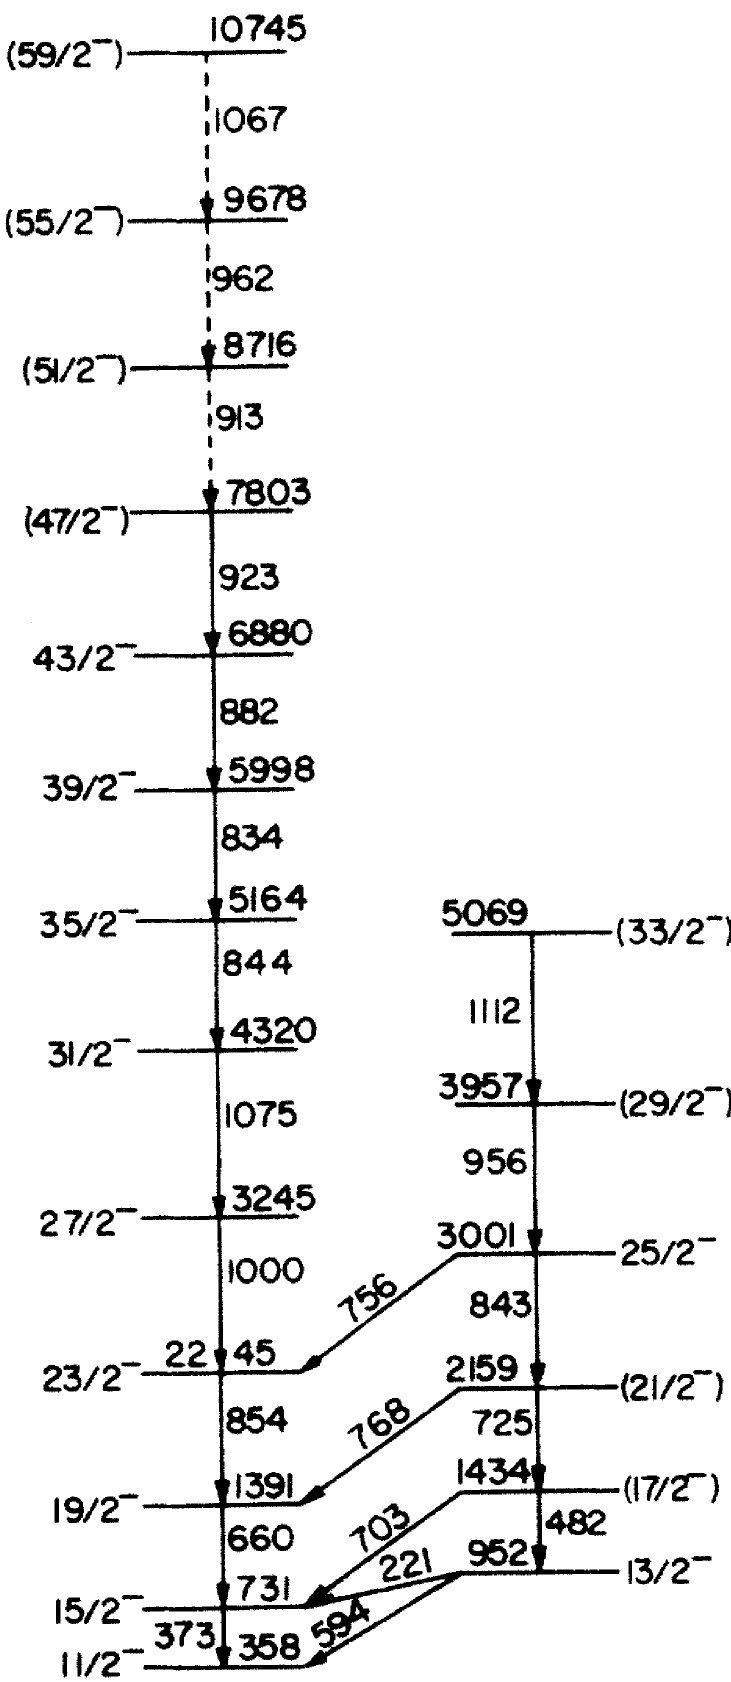
\includegraphics[height=0.4\textheight]{./img/c4/old_scheme_bands.png}\hspace{0.1\textwidth}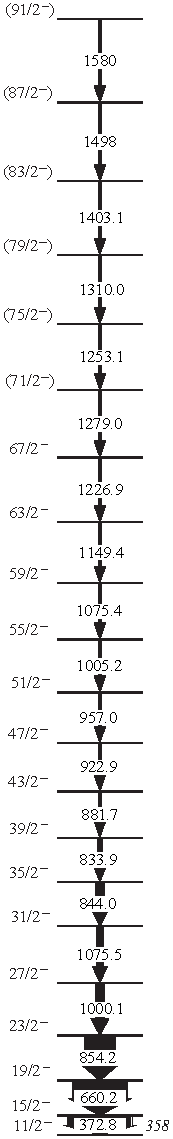
\includegraphics[height=0.4\textheight]{./img/c4/high_spin_yrast.pdf}}
	\caption{Left: Negative parity rotational band structure proposed for \pr{} in Ref. \cite{semkow135Pr}. Right: Yrast band presented in Ref. \cite{ePaul135Pr}. \label{fig:chp4-prev-bands}}
\end{figure}

Previously, T.M. Semkow \emph{et al.} performed a spectroscopic study of \pr{} in  Ref. \cite{semkow135Pr} using a $\gamma$-ray detector array consisting of four HPGe detectors with NaI escape suppression, two unsuppressed HPGe detectors, and eleven NaI counters (to provide $\gamma$-ray multiplicity selection). In this experiment $1.66\times{}10^8$ $\gamma{}$-$\gamma{}$ events were collected. Using this data, the level scheme in Fig. \ref{fig:chp4-semkow-lvl-schm}, showing both positive and negative parity levels, was developed. As the positive parity portion of the level scheme is of little interest to the wobbling excitation in \pr{}, it is neglected for the rest of this work. Later in Ref. \cite{semkow135Pr}, rotational band structures for the positive and negative parity parts of the level scheme were proposed, the left panel Fig. \ref{fig:chp4-prev-bands} contains the proposed negative parity rotational band structure. Additional work, extending the yrast band to $\sfrac{91}{2}$, was done by E.S. Paul \emph{et al.} in Ref. \cite{ePaul135Pr}. The data for the work in Ref. \cite{ePaul135Pr} was a byproduct of a high statistics measurement of $^{134}$Pr done at Gammasphere. The right panel of Fig. \ref{fig:chp4-prev-bands} contains the proposed yrast structure.


\begin{landscape}
\begin{figure}[h!]
\centerline{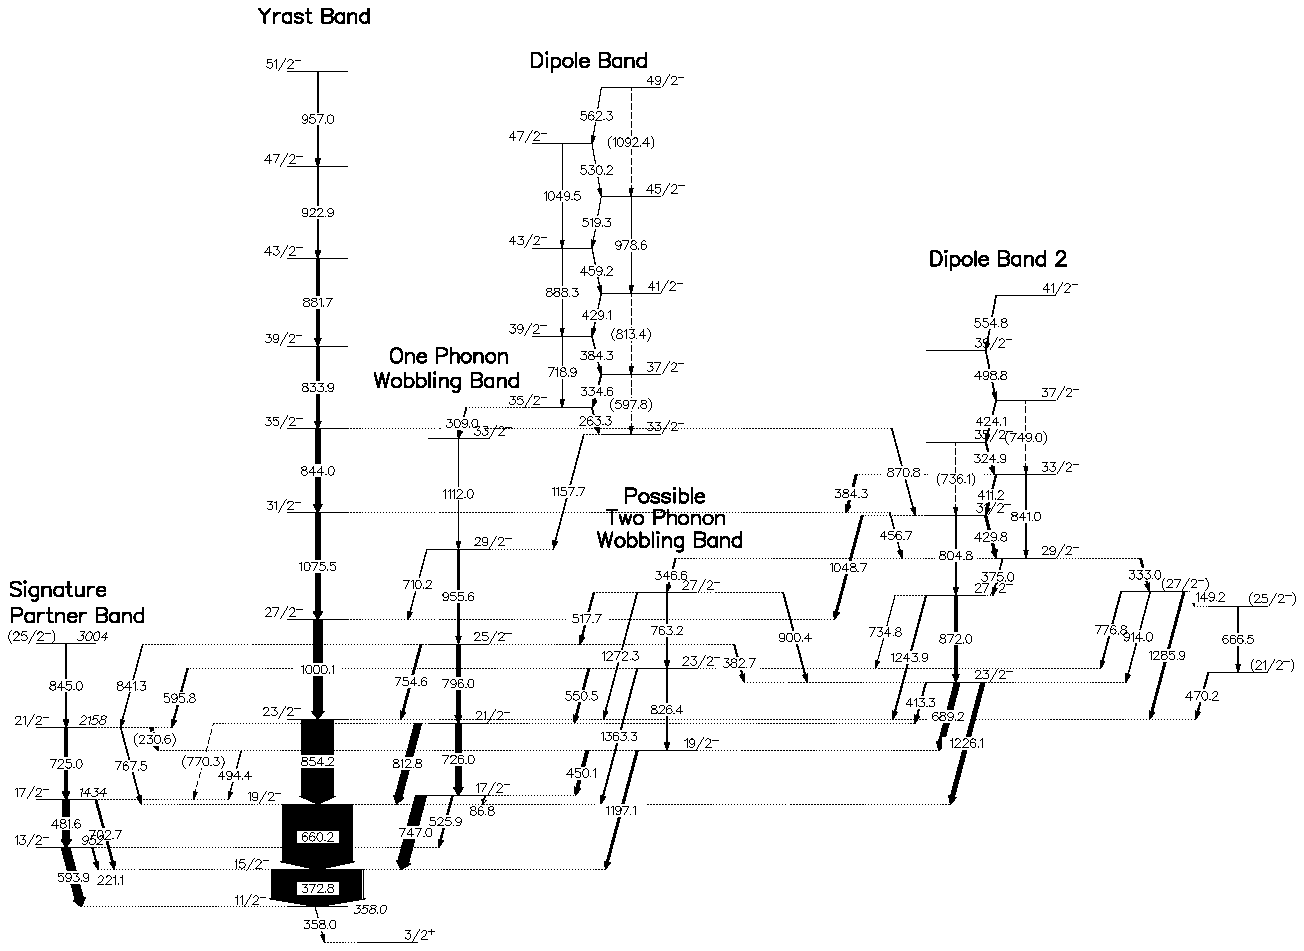
\includegraphics[height=0.9\textheight]{./img/c4/135Pr_Np_for_diss.pdf}}
	\caption{Negative parity level scheme developed for \pr{}. \label{fig:chp4-neg-par-lvl-schm}}
\end{figure}
\end{landscape}

The negative parity level scheme constructed from the Gammasphere data in this work is presented in Fig. \ref{fig:chp4-neg-par-lvl-schm}. Tables of level and transition information can be found in Appendix \ref{app:neg-par-info}. As the beam and target pair of the reaction were tuned to preferentially excite non-yrast states the yrast band was only measured to spin $\sfrac{51}{2}$. The finding of this measurement were in agreement with Ref. \cite{ePaul135Pr}. However, the band structure proposed in Ref. \cite{semkow135Pr} was in disagreement with the results found in this work. Notably, the signature partner transitions above the $\sfrac{25}{2}$ level were found to instead belong to the $n_w=1$ wobbling band. It seems that the previous work here was unable to resolve the difference between the last $845$ keV transition of the signature partner band and the $841$ keV transition linking the $n_w=1$ wobbling band to the signature partner band. Evidence for the this is given in Figs. \ref{fig:chp4-spec-dbl-gates} and \ref{fig:chp4-spec-triple-gate}. Fig. \ref{fig:chp4-spec-dbl-gates} shows the sum of the spectra resulting from every possible double gate on the dipole band. This spectrum shows the dominance of decay through the wobbling band as opposed to the signature partner band. Fig. \ref{fig:chp4-spec-triple-gate} shows a triple gate placed on the $n_w=1$ band and the dipole band immediately above the weak linking transition from the wobbling band to the signature partner band. Here the difference in the $841$ keV transition's strength and the strength of the $796$ keV transition plainly visible. This disparity in strength further highlights that the primary decay path from the $\sfrac{25}{2}$ is through the $796$ keV transition, in keeping with it being an intraband transition.

\begin{figure}[h!]
\centerline{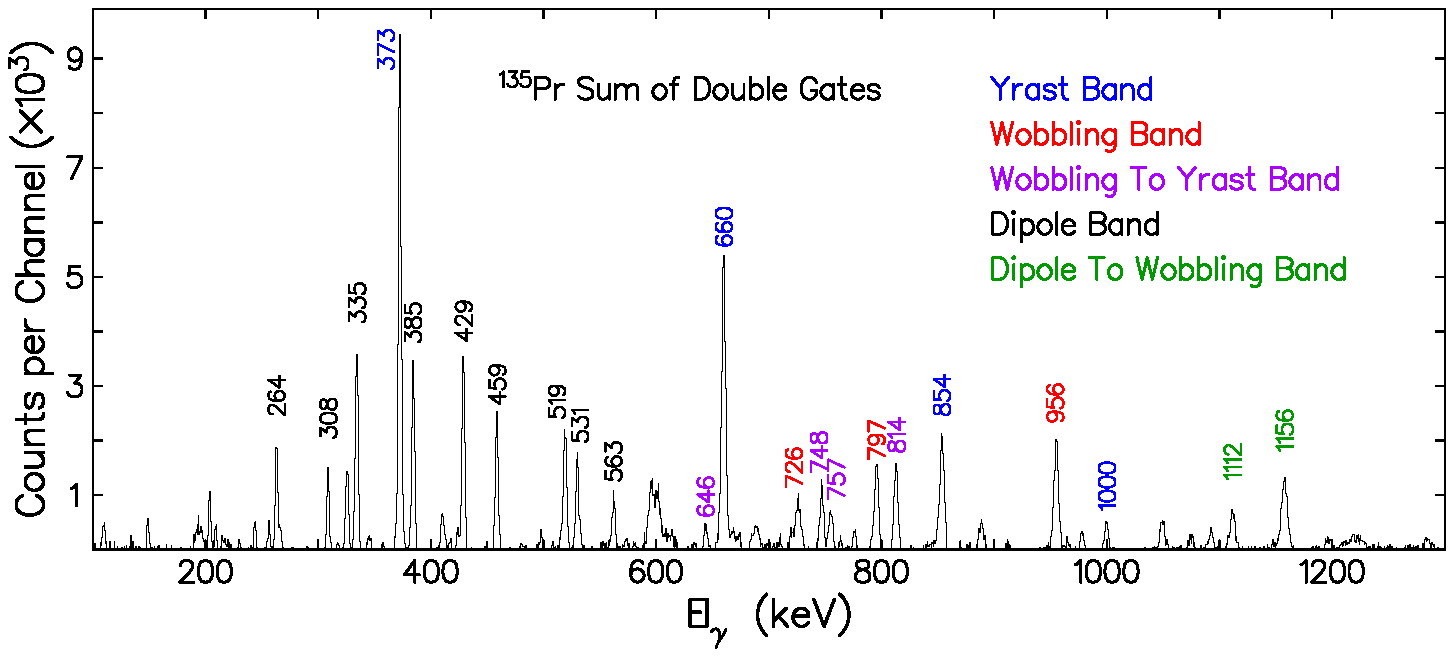
\includegraphics[width=\textwidth]{./img/c4/sum_of_dbl_gate_ev.pdf}}
	\caption{Sum of all possible double gates on M1 transitions in the dipole band. The labeling of the transitions is color coded according to the band the transition belongs to. \label{fig:chp4-spec-dbl-gates}}
\end{figure}
\begin{figure}[h!]
\centerline{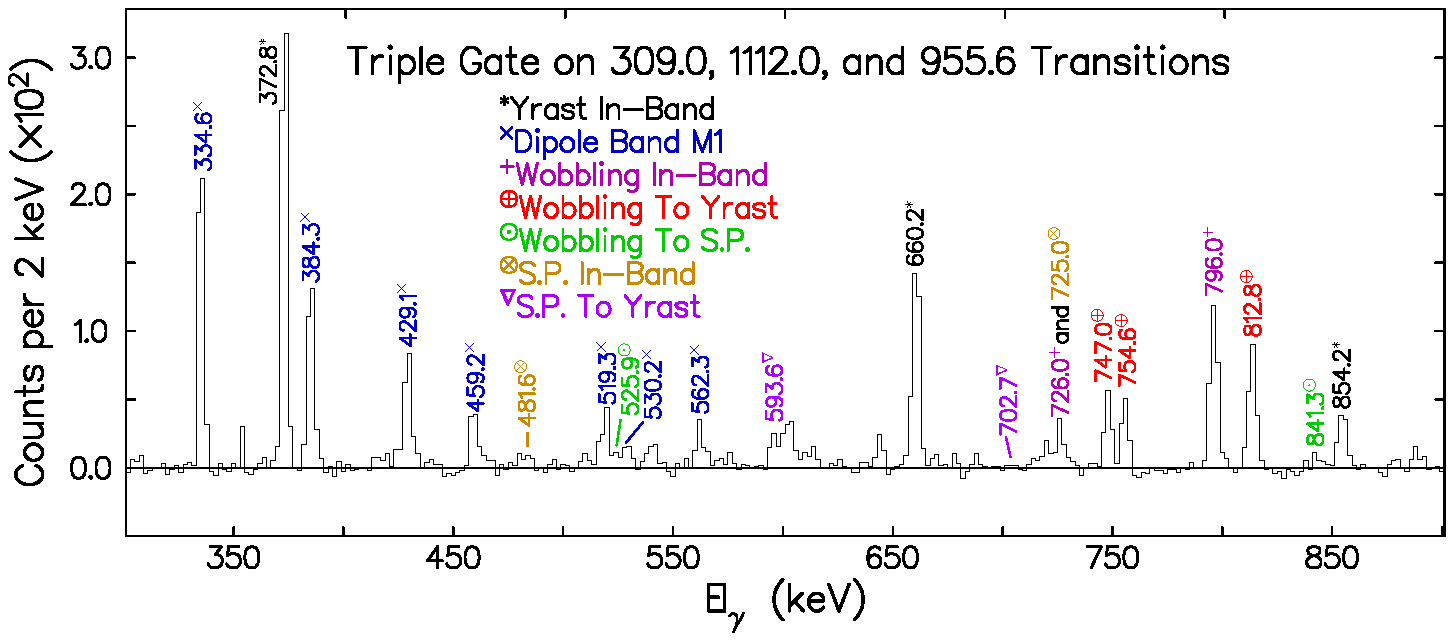
\includegraphics[width=\textwidth]{./img/c4/trip_gate_ev.pdf}}
	\caption{Sum of triple gate on the specified transitions. The labeling of the transitions is color coded according to the band the transition belongs to. \label{fig:chp4-spec-triple-gate}}
\end{figure}

Spins were assigned through the following techniques: angular distributions (method discussed in section \ref{sssec:exp-pr-data-ang-cor-dco}), DCO-like ratios (method discussed in section \ref{sssec:exp-pr-data-ang-cor-dco}) and arguments from the deexcitation of the level to multiple levels. Assignments using the first two methods are discussed in section \ref{ssec:trw-lvl-angles}; however, as the third method is relies purely on coincidence data and previously known components of the level scheme it will be addressed here.

The dipole and quadrupole transitions of Dipole Band 1 and Dipole Band 2 were assigned based on their placement. As each dipole transition (strong low energy transitions) had a cross-over transition the following reasoning was used. A cross-over transition must have a low-order multipolarity (L) equal to the sum of the low-order multipolarities of the two transitions it crosses. Therefore, a crossover of $E2$ nature is only possible if the two crossed transitions are both dipole. If one or both of the crossed transitions is of higher order then the crossing transition must be of higher order as well. Given the very low probability (slow) nature of most transitions with $L>2$ observation of the cross-over shows that the cross-over must be $E2$ and the crossed transitions $M1$. Though the top of Dipole Band 2 had cross-over transitions that were too weak to measure the observation of lower cross-over transitions and their rapidly fading strength gave confidence in the band continuing to be composed of $M1$ transitions.

The spin of dipole band 2 was fixed relative the yrast band using the four interband transitions that link the states around $\sfrac{31}{2}$ of the two bands. The pattern of linking that occurred is typical of levels that happened to mix because they were very close in energy and had the same spin and parity. Additionally, if the two apparently overlapped states were separated by one unit of angular momentum then either the $871$ keV transition or the $1049$ keV transition would have $L=3$, rendering it highly improbable. Unfortunately, this argument does not cover the $\sfrac{23}{2}$ state of dipole band 2. This state's spin was fixed by the following arguments: if the state were instead $\sfrac{21}{2}$ then the $872$ keV transition would be a highly improbable $L=3$, while if it were $\sfrac{25}{2}$ then the $689$ keV and $1226$ keV transitions would both be $L=3$, again, an improbability. The spin of the signature partner band $\sfrac{21}{2}$ level is fixed as follows. If the level were instead $\sfrac{19}{2}$, the $841$ keV transition into it would be $L=3$ in nature. Alternatively, if the level were$\sfrac{23}{2}$ then the $725$ keV transition out of it would be $L=3$. Finally, the spin of the $\sfrac{27}{2}$ was fixed as follows: If the level were $\sfrac{29}{2}$ then $1272$ keV transition would be $L=3$. Supporting the impossibility of the level being $\sfrac{25}{2}$ are these facts the $518$ keV transition would be $L=0$ which is less probable, additionally, the $1272$ keV transition would be $L=1$. If the $1272$ keV transition were $L=1$ then it could be either $M1$ or $E1$. The $M1$ possibility is highly unlikely due to rarity of $M1$ transitions with such high energy, The $E1$ possibility is countered by the large number of transitions linking the level to other negative parity levels. It would be highly improbable for the level to be of different parity from the majority of levels it connects to.

\subsection{Angular Distributions and DCO-like Ratios}
\label{ssec:trw-lvl-angles}

The first step in determining if a band is an $n_w=x$ wobbling band is to look at transitions from $n_w=x$ to $n_w=(x-1)$. For the case studied in this work, $x=1$. As stated earlier, these transitions must have $\Delta{}I=1, E2$ nature. To determine if this holds true, angular distributions of the transitions must be extracted and fitted.

Angular distributions for the first three transitions from $n_w=1\rightarrow{}n_w=0$ are plotted in the top left, top right, and middle left panels of Fig. \ref{fig:chp4-angular-distributions}. Each panel contains a plot of the extracted data, a plot of the fit to the data, and plots of the distributions for pure transitions of higher and lower order. As can be seen in the figures the angular distributions for the $n_w=1\rightarrow{}n_w=0$ transitions are strongly mixed with the higher order nature. The shows that the transitions are $\Delta{}I=1, L=2$, while it is highly probably that the polarization of the transition is $E$, to \emph{guarantee} that the transition is $E2$ polarization measurements are necessary. The middle right panel of Fig. \ref{fig:chp4-angular-distributions} holds the angular distribution of the first transition from the band identified as a possible $n_w=2$ band to the $n_w=1$ band. As can be seen in the figure, this distribution is also highly mixed. This is a hopeful sign that the band is in fact the $n_w=2$ band. 

To ensure that the signature partner to yrast transitions are of substantially different character, the bottom left panel of Fig. \ref{fig:chp4-angular-distributions} contains the angular distribution of the first signature partner to yrast transition. Examination of this transition shows that it is less than $3\%~E2$, as expected of signature partner to yrast transition. As an additional check on the angular distribution extraction and fitting procedure the
\begin{figure}[t!]
\centerline{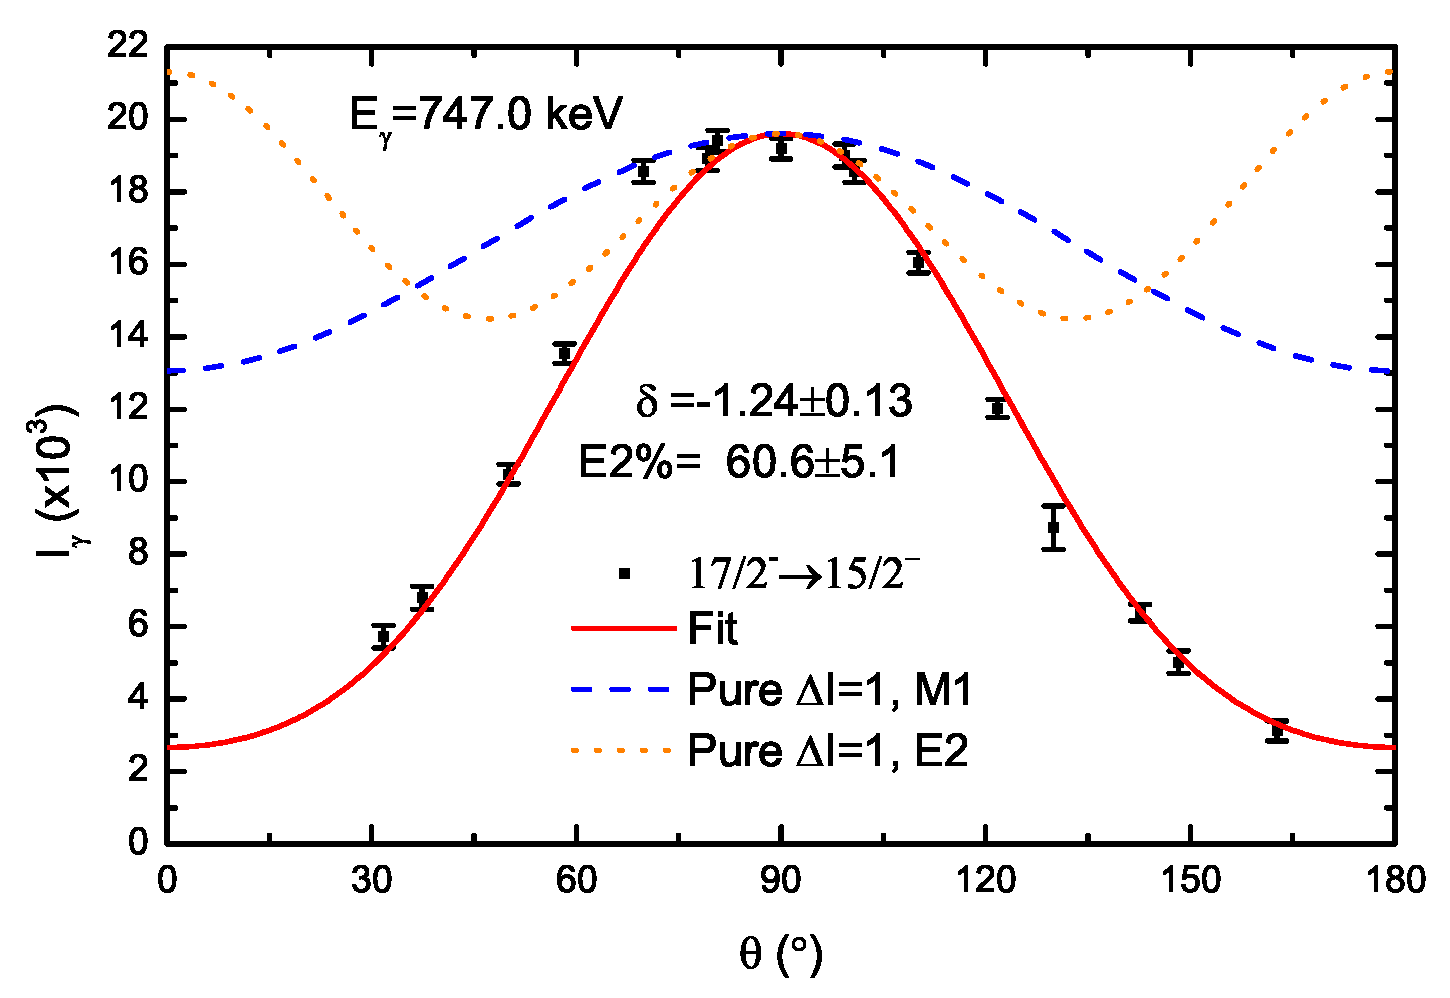
\includegraphics[width=0.475\textwidth]{./img/c4/747Dist_Plot.eps}\hspace{0.04\textwidth}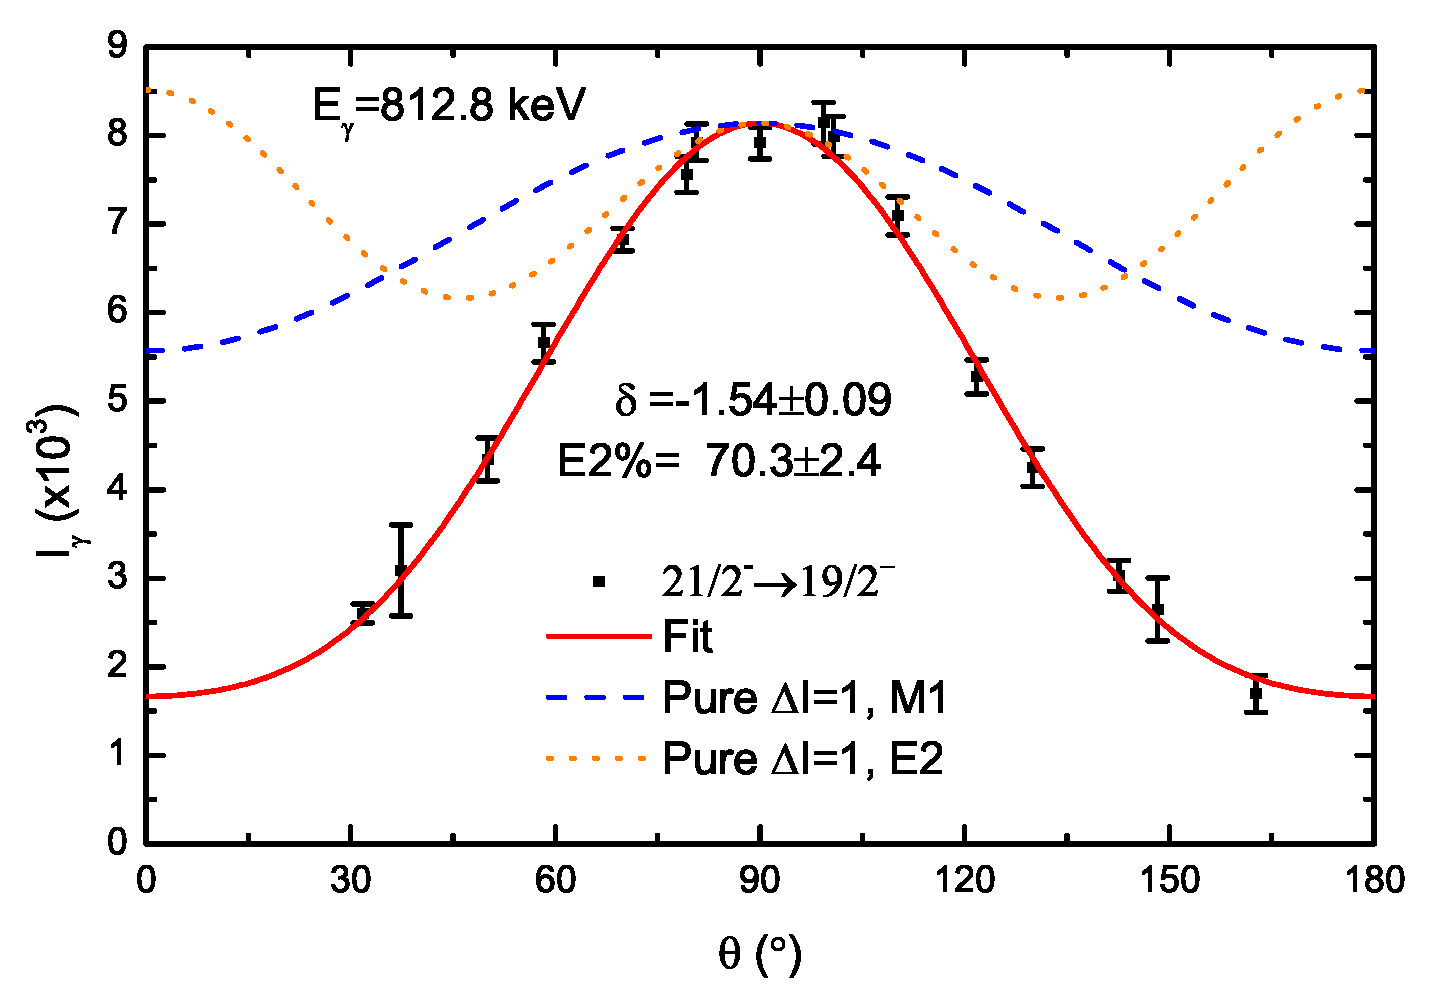
\includegraphics[width=0.475\textwidth]{./img/c4/813Dist_Plot.eps}}
\centerline{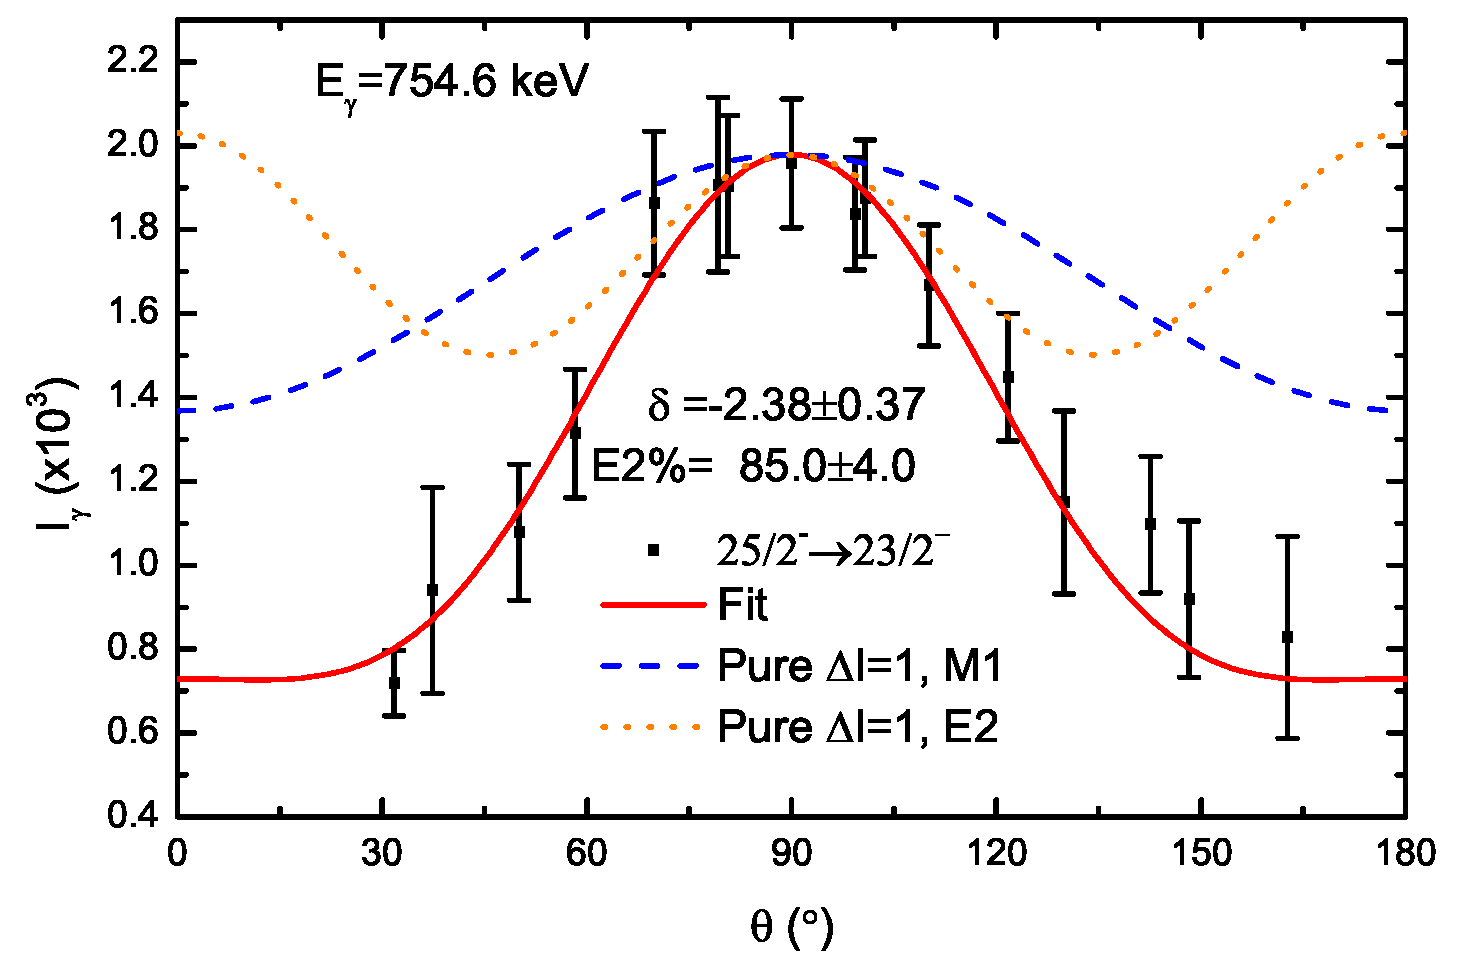
\includegraphics[width=0.475\textwidth]{./img/c4/755Dist_Plot.eps}\hspace{0.04\textwidth}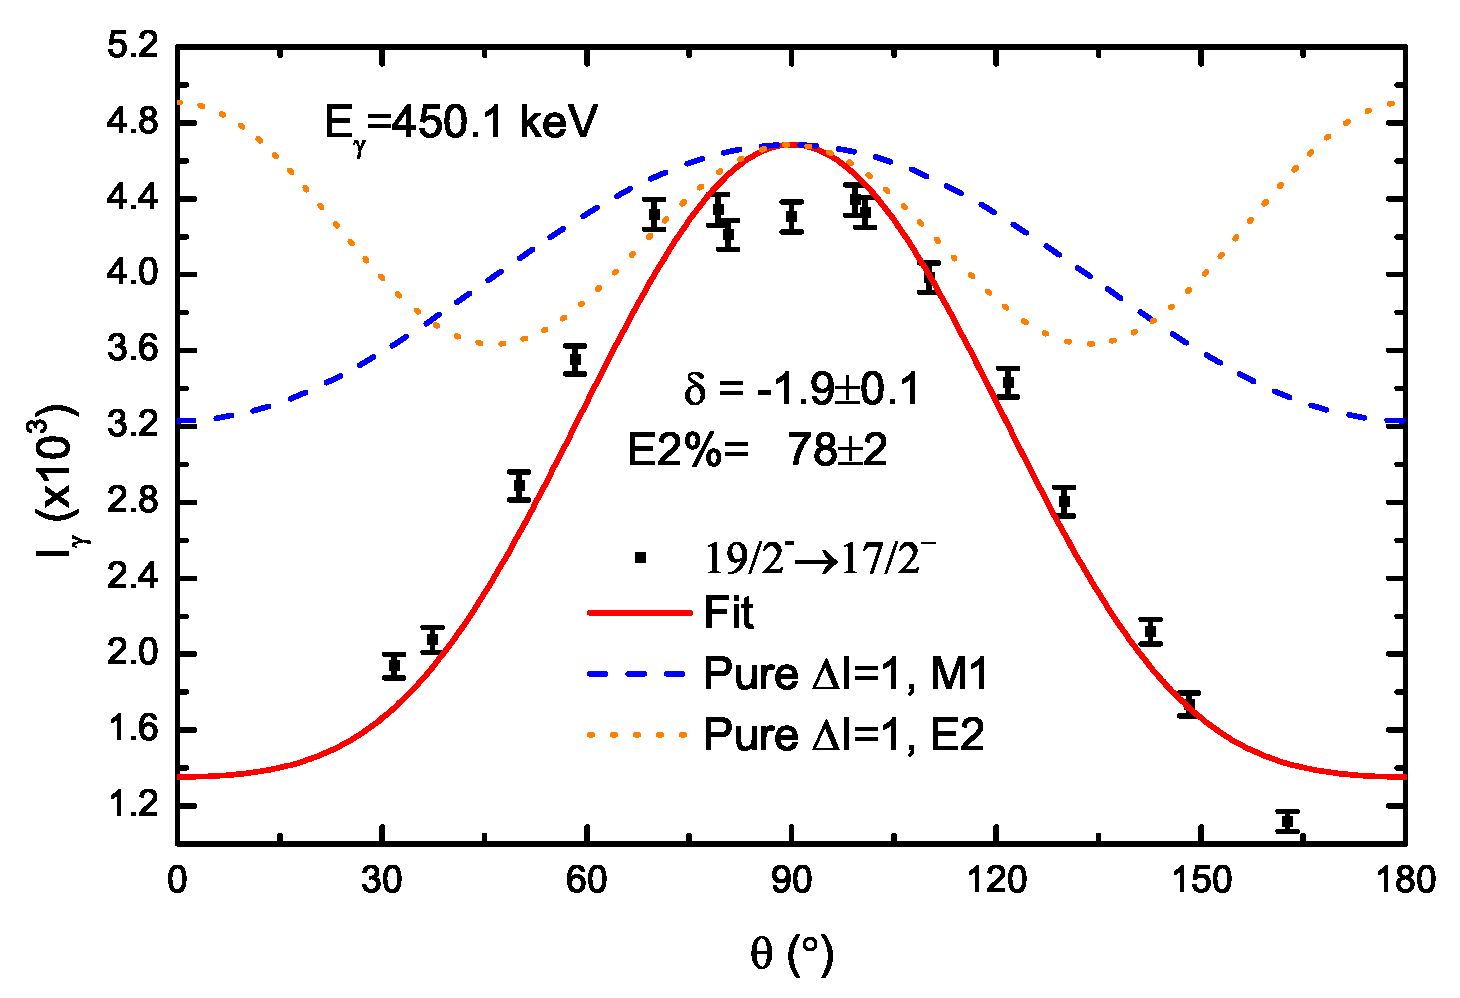
\includegraphics[width=0.475\textwidth]{./img/c4/450Dist_Plot.eps}}
\centerline{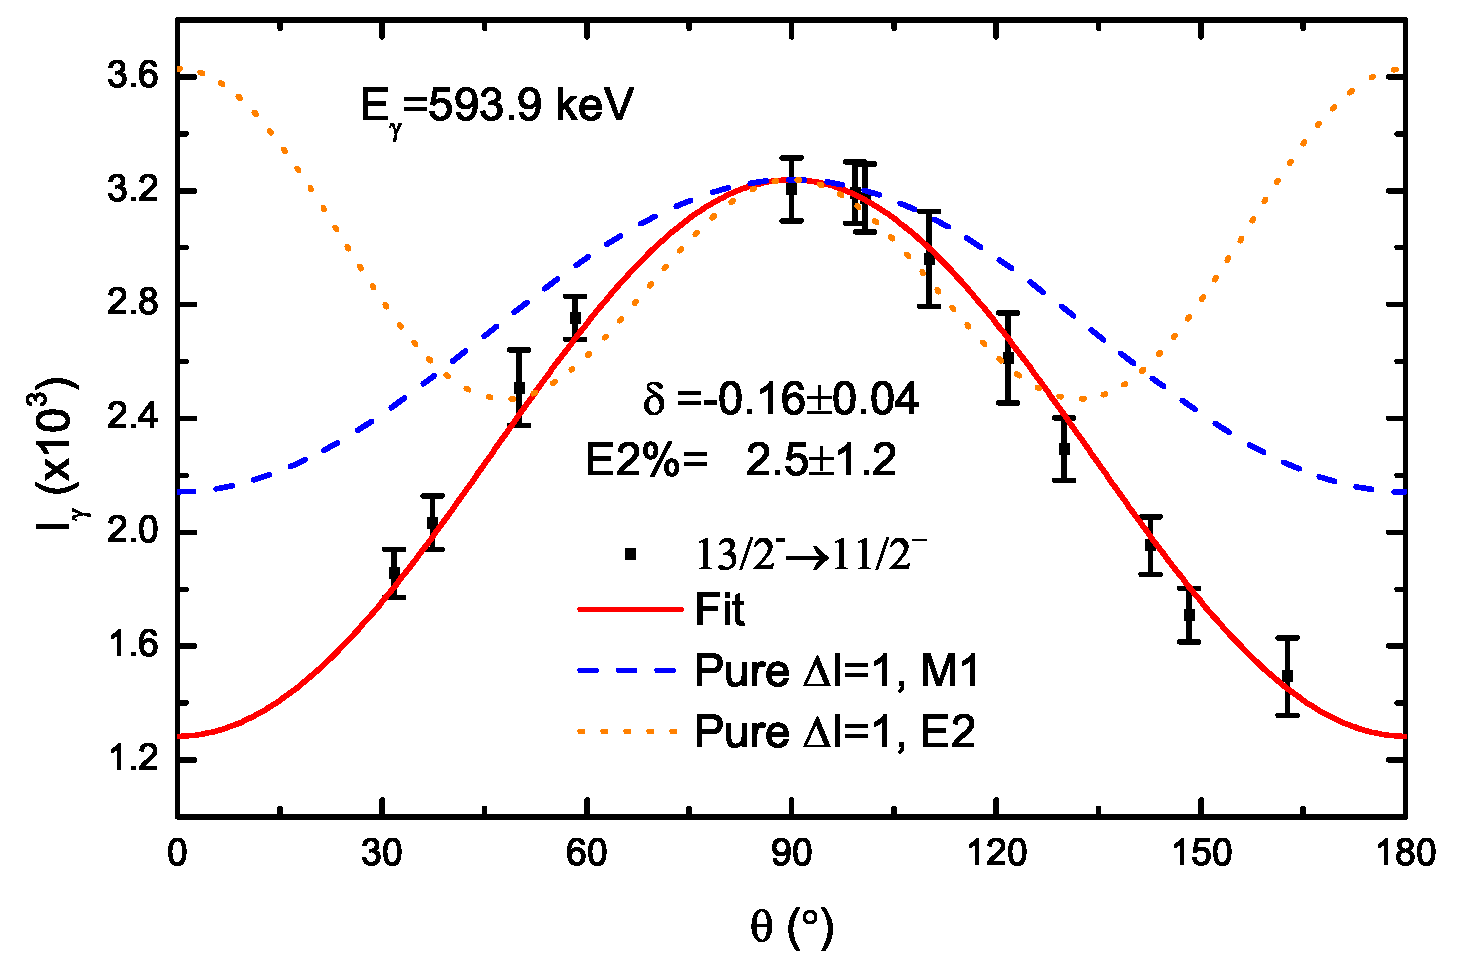
\includegraphics[width=0.475\textwidth]{./img/c4/594Dist_Plot.eps}\hspace{0.04\textwidth}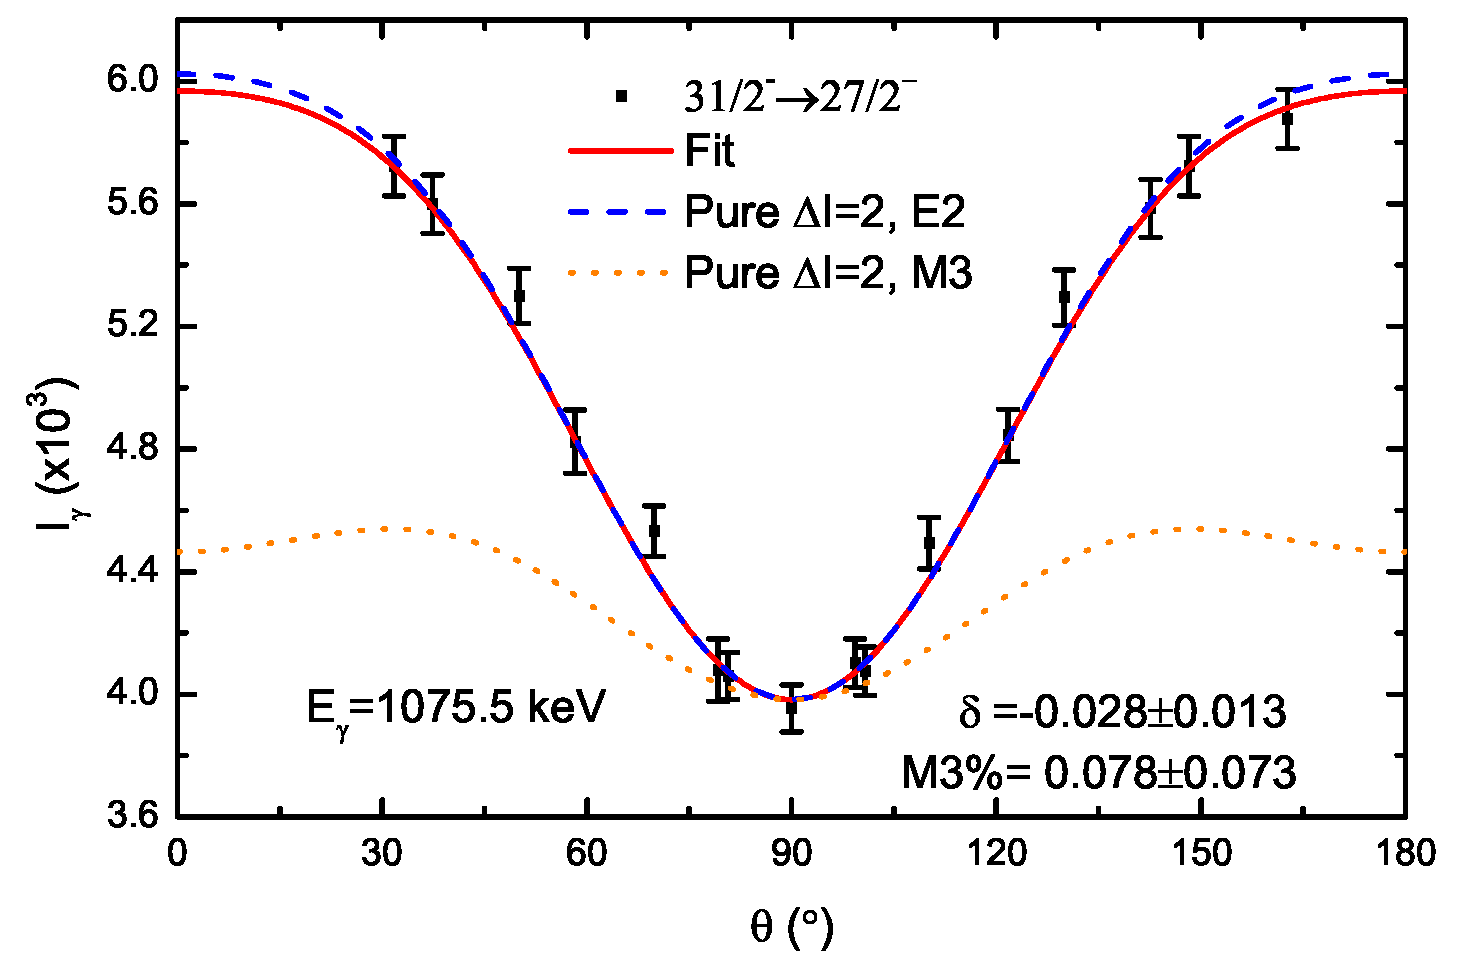
\includegraphics[width=0.475\textwidth]{./img/c4/1075Dist_Plot.eps}}
	\caption{Important angular distributions fitted in this work. Top Left: The first $n_w=1\rightarrow{}n_w=0$ transition ($747.0$ keV). Top Right: The second $n_w=1\rightarrow{}n_w=0$ transition ($812.8$ keV). Mid Left: The third $n_w=1\rightarrow{}n_w=0$ transition ($754.6$ keV). Mid Right: The first possible $n_w=2\rightarrow{}n_w=1$ transition ($450.1$ keV).  Bottom Left: The first signature partner to yrast transition ($593.9$ keV). Bottom Right: The fifth yrast in-band transition ($1075.5$ keV).\label{fig:chp4-angular-distributions}}
\end{figure}
angular distribution of the fifth yrast in-band transition. As it's nature is $\Delta{}I=2, E2$, substantially different from the transitions fitted previously, flaws in the procedure that may be hidden for $\Delta{}I=1$ transitions should be more easily visible. As shown in the bottom right panel of Fig. \ref{fig:chp4-angular-distributions}, this check revealed no issues, as expected the transition was found to be pure $E2$ in nature.
 
Angular distributions provide a highly detailed examination of a transitions multipolarity; however, because any gates to clean the resultant spectra must be placed below the transition of interest, and because the intensity of the transition is distributed across many rings, they can be difficult and time consuming to extract. As mentioned in section \ref{sssec:exp-pr-data-ang-cor-dco} DCO-like ratios are a convenient method for extracting the multi-polarity of the distribution. While it is much harder to get a good limit on the mixing ratio $\delta$ with this method, in cases where this is not necessary the higher intensity and fewer values to fit and extract make the DCO-like ratio a very useful method to extract transition multipolarity. Table \ref{tbl:chp3-dco-ratios} gives the values of the DCO-like ratio associated with each multipolarity. 

Fig. \ref{fig:chp4-dco} contains a plot of many of the DCO ratios measured for this nucleus. The $372.8$ keV and $660.2$ keV transitions of the yrast band, known to be very pure quadrupole transitions have values slightly lower than expected for a combination of two reason. The first is that these transitions are so intense that their peaks become very hard to fit due to strange contributions of width from detectors at different angles to the beam axis. The second reason is that the DCO-like ratios presented in Table \ref{tbl:chp3-dco-ratios} and drawn on Fig. \ref{fig:chp4-dco} were computed for a substate distribution width of $\sigma{}=0.3J_i$. While this is quite close to true (and thus a reasonable approximation) two transitions above the $372.8$ keV transition, this approximation breaks down somewhat at the lower spin where the substate distribution width drops to $\sigma{}=0.23J_i$. Nevertheless the values are still in decent agreement with quadrupole transitions.

Examination of Fig. \ref{fig:chp4-dco} reveals that the DCO-like ratios of the $n_w=1\rightarrow{}n_w=0$ transitions are as expected of highly mixed transitions with negative mixing ratio. Further, the DCO-like ratio for the $710.2$ keV transition was extracted and shown to be highly mixed, confirming the trend established in the previous $n_w=1\rightarrow{}n_w=0$ transitions. Additionally, the DCO-like ratio of the first possible $n_w=2\rightarrow{}n_w=1$ transition confirms the angular distribution and the ratio of the second possible $n_w=2\rightarrow{}n_w=1$ transition shows the trend of highly mixed possible $n_w=2\rightarrow{}n_w=1$ transitions continuing.

\begin{figure}[t!]
\centerline{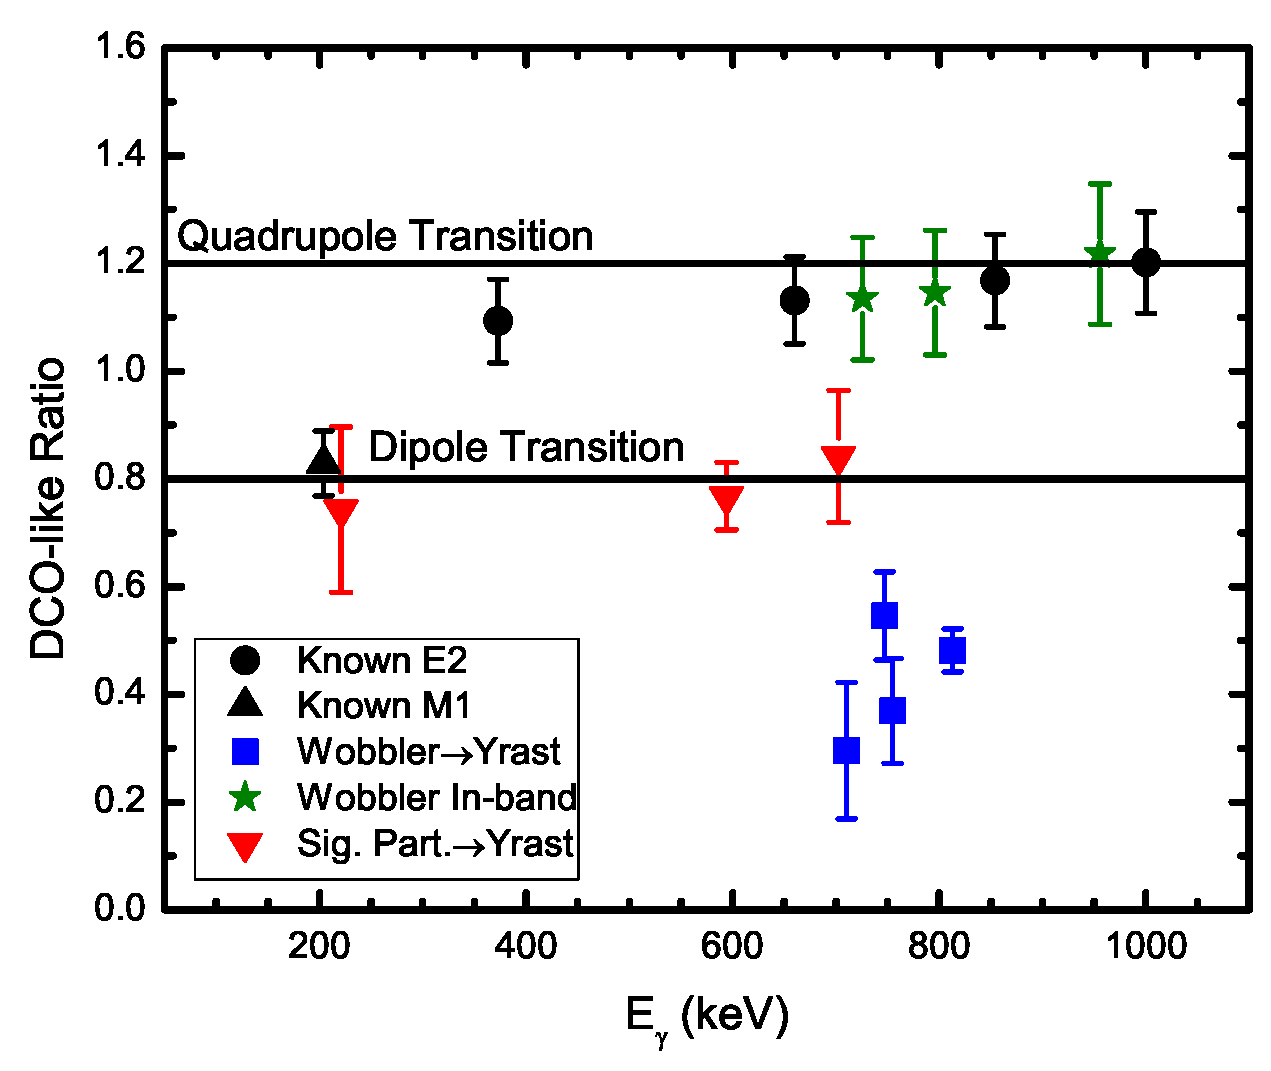
\includegraphics[width=\textwidth]{./img/c4/DCO.eps}}
	\caption{DCO-like ratios plotted versus transition energy for a wide variety of transitions in \pr{}.\label{fig:chp4-dco}}
\end{figure}

With the angular distributions and DCO-like ratios the spins of the $n_w=1$ band, $n_w=2$ band, signature partner band, and dipole band 1 can be fixed relative to the yrast spins. The DCO ratios of the $309$ keV transition and the $1157.7$ keV transitions from dipole band 1 to the $n_w=1$ band firmly lock its spin relative to the wobbling band. In turn the angular distributions and the DCO-like ratios of the $n_w=1\rightarrow{}n_w=0$ transitions lock the wobbling band relative to the yrast band. The DCO-like ratios and angular distributions of the signature partner to yrast band transitions lock the spins of the signature partner states relative to the yrast band. The final set of spins to fix, the possible $n_w=2$ band, are fixed by the angular distribution of the bottom transition to the $n_w=1$ band, by the DCO-like ratios of the bottom and middle transition to the $n_w=1$ band, and finally by the arguments given in the last paragraph of section \ref{sec:trw-lvl-scheme}

\section{Polarizations}
\label{ssec:trw-lvl-pol}

It is highly probable that the polarization of the $n_w=1\rightarrow{}n_w=2$ transitions is electric in nature; however, to absolutely guarantee this it is necessary to measure polarizations. As described in section \ref{ssec:exp-pol} polarizations of transitions can be extracted using arrays of clover type HPGE detectors. To this end an experiment was performed at the INGA array \cite{ingaAtIUAC,ingaAtIuacConf} located at the Tata Institute for Fundamental Research in Mumbai, India.

The data from this experiment were sorted into two asymmetric matrices (E$_{\gamma}$-E$_{\gamma}$) using the code MARCOS \cite{IngaDigitalDAQ}. The first of these matrices consisted of all gamma-ray events where at least one of the gamma-rays scattered perpendicular to the reaction plane on the y-axis and the other gamma energy (with no restrictions) on the x-axis. The second of these matrices consisted of all gamma-ray events where at least one of the gamma-rays scattered parallel to the reaction plane on the y-axis. With these matrices and the correction to the asymmetry due to the geometry of the array (denoted $a$, see section \ref{ssec:exp-pol} for details) asymmetries for transitions can be extracted. If the asymmetry is positive then the transition had electric nature, contrariwise, if the transition has magnetic nature, then the asymmetry is negative.

\begin{figure}[t!]
\centerline{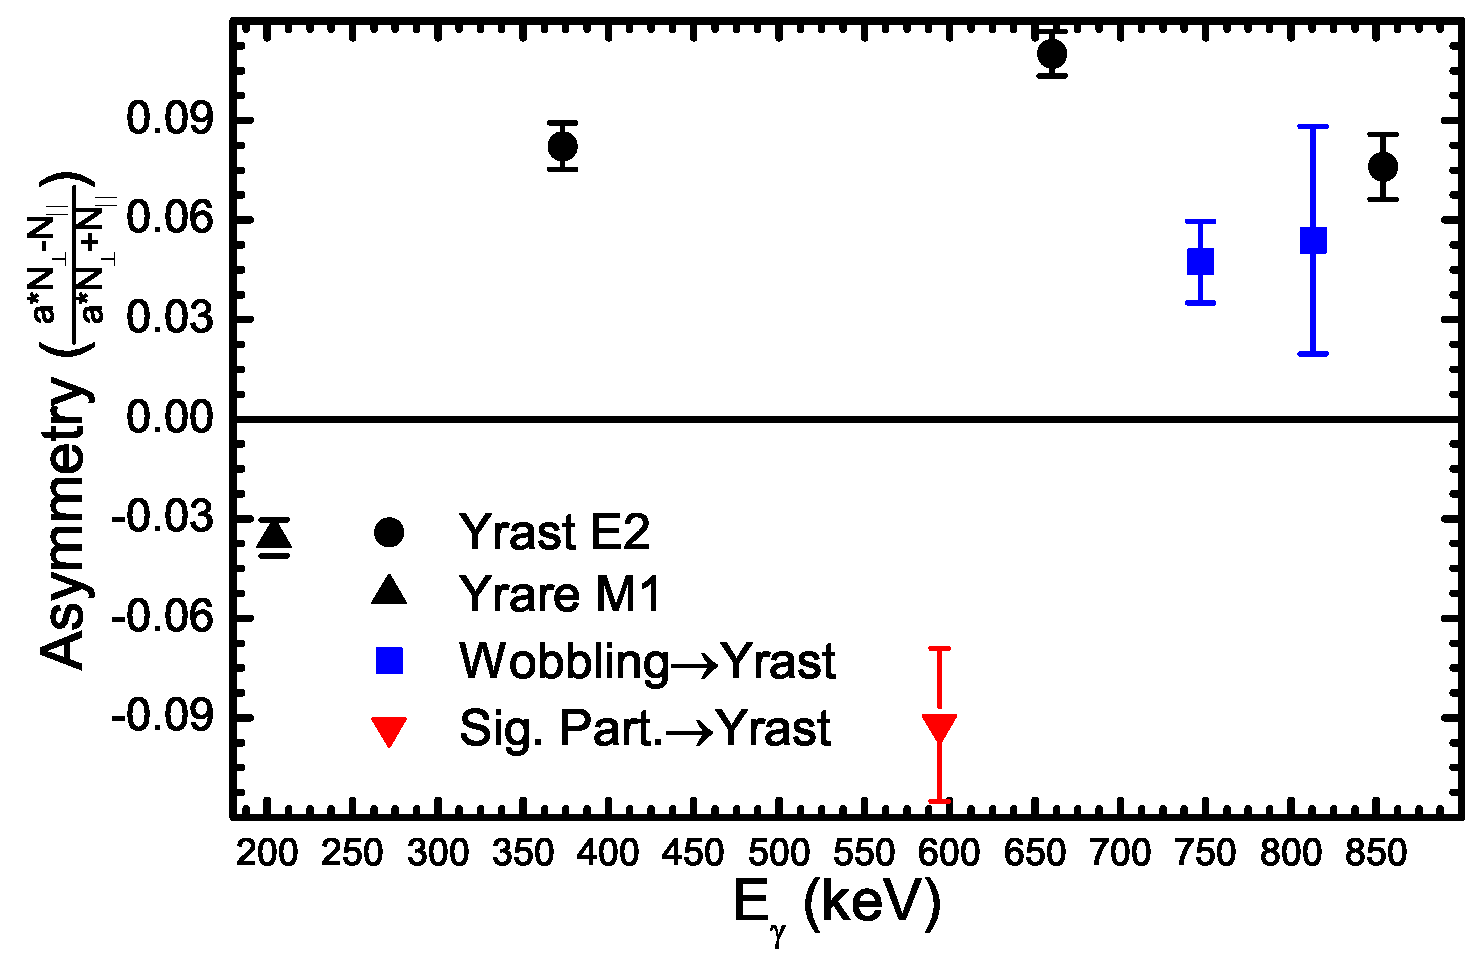
\includegraphics[width=\textwidth]{./img/c4/AsymPlot.eps}}
	\caption{Polarization asymmetries versus transition energy for several transitions in \pr{}.\label{fig:chp4-asyms}}
\end{figure}

Due to the thick target and poorer statistics of the INGA experiment relative to the Gammasphere experiment, only the bottom two $n_w=1\rightarrow{}n_w=0$ transitions had extractable polarization asymmetries. Despite this, these asymmetries show that the transitions are definitely electric in nature confirming the $\Delta{}I=1, E2$ nature of the transitions. Given this the $n_w=1$ wobbling band is confirmed and the case is strong for the possible $n_w=2$ wobbling band. The angular distribution and polarization asymmetry results for the $n_w=1$, possible $n_w=2$, and signature partner bands are summarized in Table \ref{tbl:chp4-mixing-asym}. This table contrains the polarization asymmetries, mixing ratios, $E2$ percentages for the wobbling transitions and the bottom most signature partner to yrast band transitions. 

\begin{table*}
\begin{center}
\caption{TABLE OF EXTRACTED MIXING RATIOS, POLARIZATION ASYMMETRIES, AND $E2$ PERCENTAGES FOR THE $n_w=1$, POSSIBLE $n_w=2$, AND SIGNATURE PARTNER BANDS.\label{tbl:chp4-mixing-asym}}
\begin{tabular}{|c|c|c|c|c|c|}
\hline
\hline
Initial $I^\pi{}$ &$E_{\gamma}$ (keV) &$\delta$ & Asymmetry & \% E2 & DCO-like\\
\hline
$\frac{17}{2}^-$ & 747.0 & $-1.24\pm0.13$ & $0.047\pm0.012$ & $60.6\pm5.1$ & $0.546\pm0.082$\\
$\frac{21}{2}^-$ & 812.8 & $-1.54\pm0.09$ & $0.054\pm0.034$ & $70.3\pm2.4$ & $0.482\pm0.040$\\
$\frac{25}{2}^-$ & 754.6 & $-2.38\pm0.37$ & -- & $85.0\pm4.0$ & $0.369\pm0.098$\\
$\frac{29}{2}^-$ & 710.2 & -- & -- & -- & $0.296\pm0.127$\\
\hline
$\frac{19}{2}^-$ & 450.1 & $-1.54\pm0.09$ & -- & $78\pm2$ & $0.50\pm0.15$\\
$\frac{23}{2}^-$ & 550.5 & -- & -- & -- & $0.48\pm0.23$\\
\hline
$\frac{13}{2}^-$ & 593.9 & $-1.90\pm0.1$ & $-0.092\pm{}0.023$ & $2.5\pm1.2$ & $0.77\pm0.06$\\
$\frac{13}{2}^-$ & 221.1 & $0.23\pm0.03$ & -- & $5.0\pm1.2$ & $0.74\pm0.15$\\
$\frac{17}{2}^-$ & 702.7 & -- & -- & -- & $0.84\pm0.12$\\
\hline
\hline\end{tabular}
\end{center}
\end{table*}

\section{Description By Theory}
\label{sec:trw-theory-desc}
Theoretical calculations within the framework of the QTR and TAC models to describe the $n_w=1$ band, the signature partner band, dipole band 1, and the yrast band in \pr{} were performed by S. Frauendorf and F. D\"onau in Ref. \cite{frauendorfTransverseWobbling}. Updated calculations were performed by S. Frauendorf and W. Li in Ref. \cite{mattaTransversePRL}. Experimental level energies, wobbling energies, and reduced transition probability ratios were compared and against these calculations.

For the QTR calculations the triaxial rotor is parameterized by three angular momentum dependent MOI with the form $\mathcal{J}_i=\Theta_i(1+cI)$ with $i=m,s,l$, denoting the short medium and long axes respectively. Adjusting the QTR energies to the experimental energies of the yrast and $n_w=1$ bands the parameters used were $\mathcal{J}_m,\mathcal{J}_s,\mathcal{J}_l = 7.4, 5.6, 1.8 \hbar{}/MeV$ and $c=0.116$. The QTR model was then used to calculate state energies, wobbling energies and reduced transition probability ratios. Fig. \ref{fig:chp4-wobb-en} contains a plot of the wobbling energy calculated from the QTR model compared against the experimental wobbling energy. Fig \ref{fig:chp4-qtr-en-minus-rotor} contains a plot of QTR and experimental level energies with a $0.02\times{}I(I+2)$ rigid rotor component subtracted. A table of experimental and QTR reduced transition probability ratios can be found in Table \ref{tbl:chp4-transitition-ratios}. Plots of the experimental and theoretical values of $B(M1_{out})/B(E2_{in})$ can be found in the left panel of Fig. \ref{fig:chp4-trans-prob-ratios}, the correspond plots for $B(E2_{out})/B(E2_{in})$ can be found in the right panel. Experimental reduced transition probability ratios are calculated using the formula from Ref. \cite{exoticNuclearExcitations}:
\begin{align}
\label{eqn:chp4-red-trans-prob-ratios}
\frac{B(M1_{out})}{B(E2_{in})} &= 0.697 \frac{E_{\gamma}(E2_{in})^5}{E_{\gamma}(M1_{out})^3}\frac{1}{(1+\delta^2)\lambda{}_{E2_{In}/M1_{out}}}\\
\frac{B(E2_{out})}{B(E2_{in})} &= \frac{E_{\gamma}(E2_{in})^5}{E_{\gamma}(E2_{out})^5}\frac{\delta^2}{(1+\delta^2)\lambda{}_{E2_{In}/E2_{out}}}
\end{align}
Here, $\lambda{}_{X1/X2}$ is the branching ratio, or intensity ratio of the transition ($X1$) to the transition ($X2$) and $\delta$ is the mixing ratio extracted from an angular distribution measurement.

\begin{figure}[t!]
\centerline{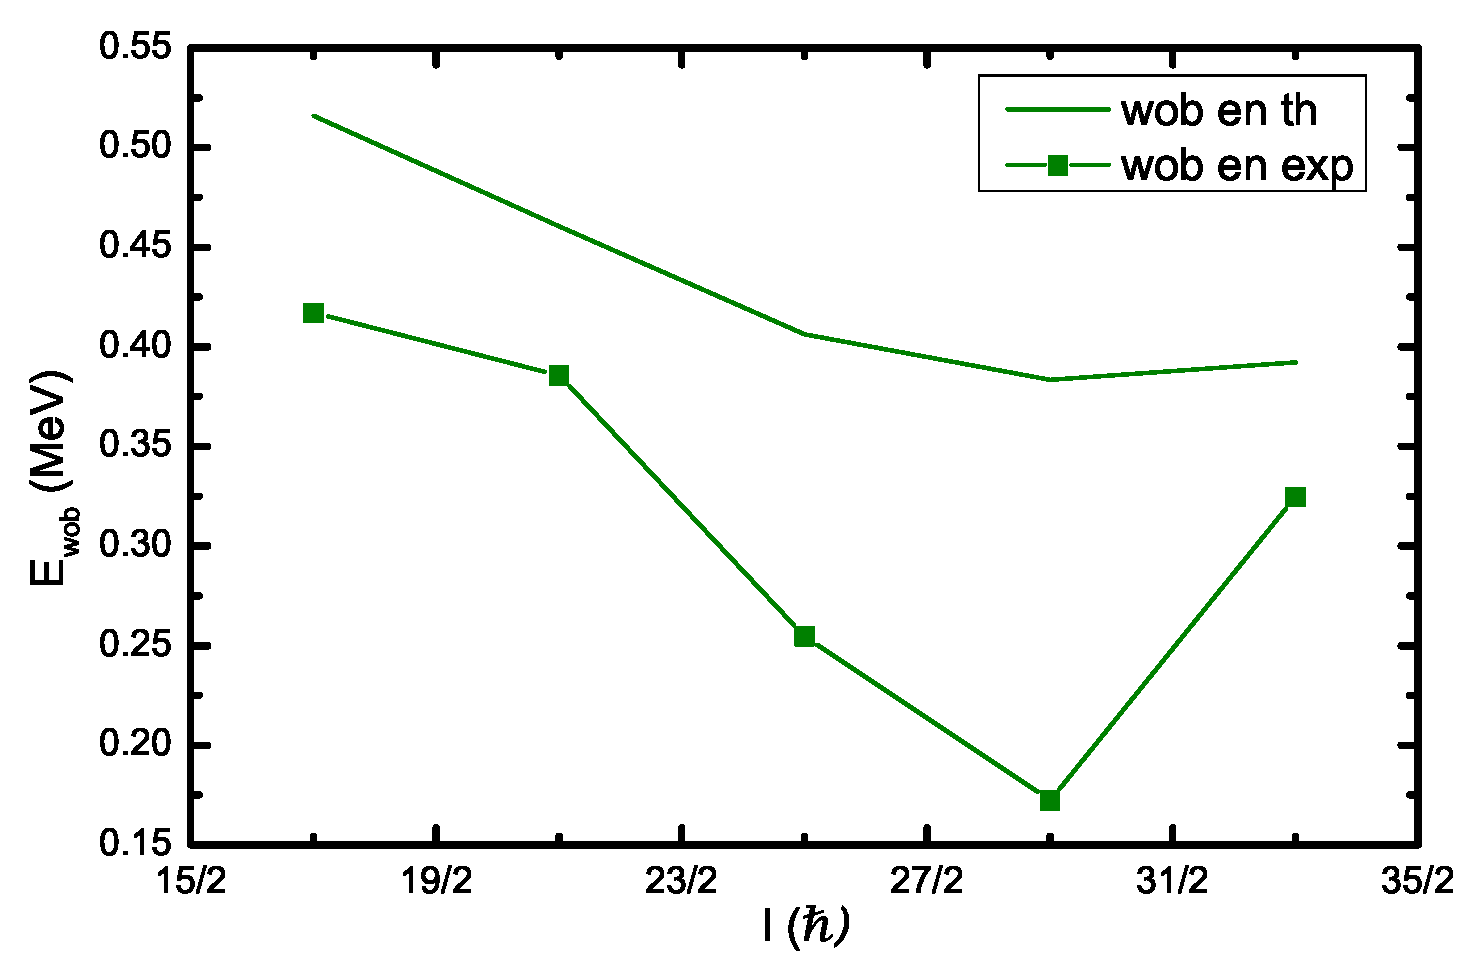
\includegraphics[width=\textwidth]{./img/c4/wob_en.eps}}
	\caption{Wobbling energies from experiment and QTR theory of the $n_w=1$ band.\label{fig:chp4-wobb-en}}
\end{figure}

\begin{figure}[b!]
\centerline{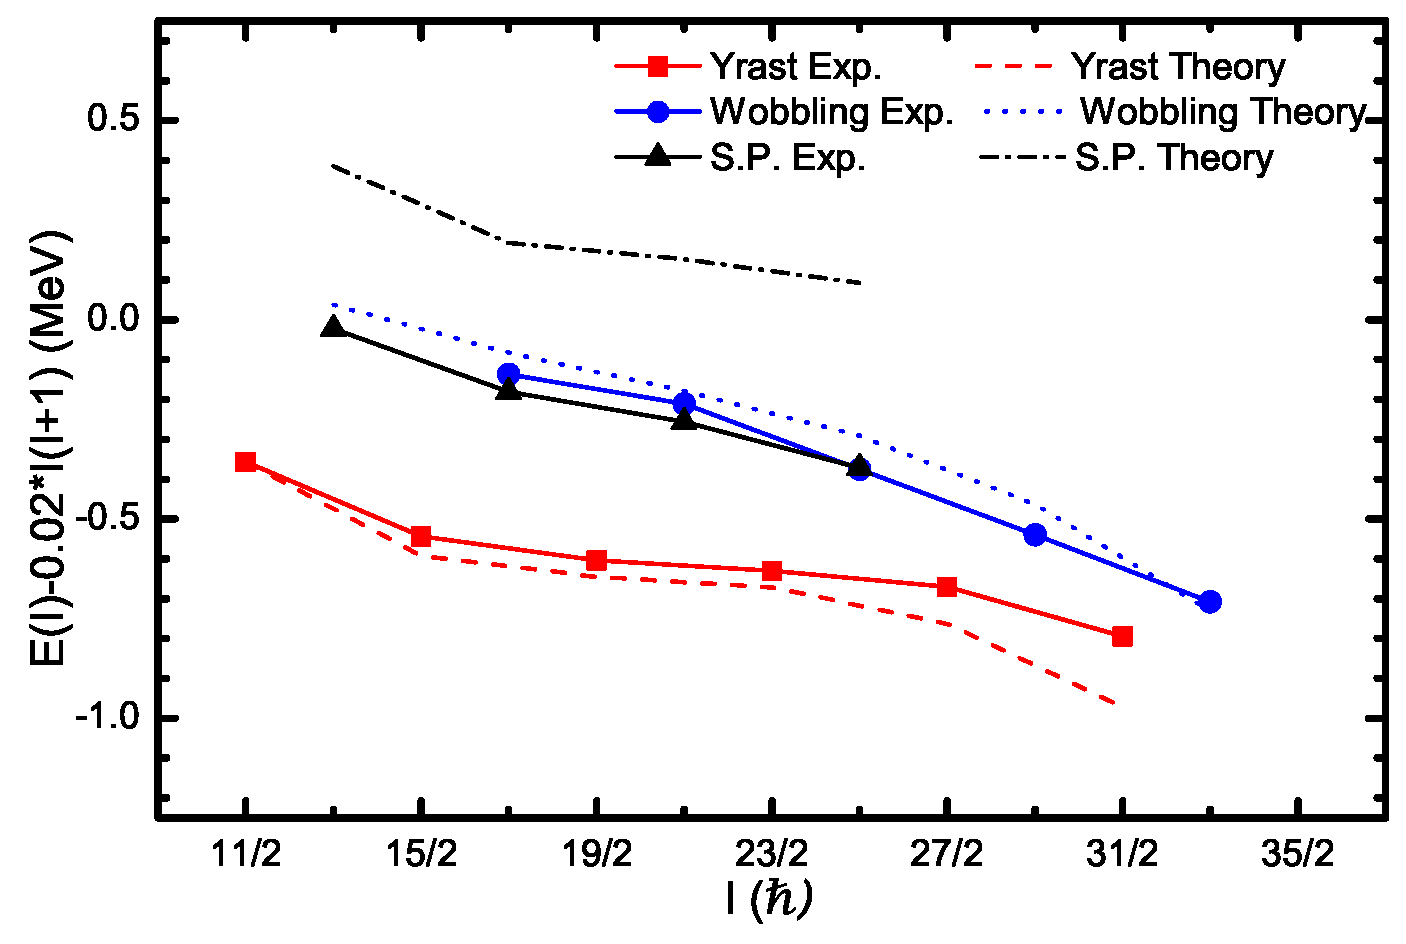
\includegraphics[width=\textwidth]{./img/c4/en_minus_rotor.eps}}
	\caption{Wobbling energies from experiment and QTR theory of the $n_w=1$ band.\label{fig:chp4-qtr-en-minus-rotor}}
\end{figure}

As shown in Fig. \ref{fig:chp4-wobb-en} the QTR model reproduces the experimental data well showing the minimum in $E_{wobb}$ at $I^{\pi}=\sfrac{29}{2}^-$ and the subsequent upturn. This upturn is due to the coriolis force detaching the quasiproton from the short axis and aligning it to the intermediate axis, switching the system from transverse to longitudinal wobbling. Regrettably QTR does not reproduce the size of the upturn seen in experiment because, simultaneous to the realignment in the wobbling band, the yrast band is undergoing a transition from a $\pi(h_{11/2}$ configuration to a $\pi(h_{11/2}^3\nu(h_{11/2}^2$ configuration (in agreement with Ref. \cite{ePaul135Pr}). The level energies in Fig. \ref{fig:chp4-qtr-en-minus-rotor} for the yrast and wobbling bands are in good agreement with experiment, but the theory predicted signature partner band $\sim0.5$MeV above its experimental counterpart. Happily TAC calculations, discussed in more detail shortly, reproduce the signature partner band well.

\begin{table*}
\begin{center}
\caption{TABLE OF REDUCED TRANSITION PROBABILITIES CALCULATED FROM DATA AND FROM QTR THEORY FOR THE $n_w=1 \rightarrow n_w=1$ TRANSITIONS.\label{tbl:chp4-transitition-ratios}}
\begin{tabular}{|c|c|c|c|c|c|}
\hline
Initial $I^\pi{}$ &$E_{\gamma}$ (keV) & \multicolumn{2}{c|}{ $\frac{B(M1_{out})}{B(E2_{in})}(\frac{\mu_N^2}{e^2b^2})$} & \multicolumn{2}{c|}{$\frac{B(E2_{out})}{B(E2_{in})}$} \\
& & Experiment & QTR & Experiment & QTR \\
\hline
$\frac{17}{2}^-$ & 747.0 & -- & $0.213$ & -- & $0.908$ \\
$\frac{21}{2}^-$ & 812.8 &  $0.164\pm0.014$ & $0.107$ &  $0.843\pm0.032$ & $0.488$ \\
$\frac{25}{2}^-$ & 754.6 &   $0.035\pm0.009$ & $0.070$ &  $0.500\pm0.025$ & $0.290$ \\
$\frac{29}{2}^-$ & 710.2 & $\leq0.016\pm0.004$ & $0.056$ & $\geq 0.261\pm0.014$ & $0.191$ \\
$\frac{33}{2}^-$ & -- & -- & $0.048$ & -- & $0.131$ \\
\bottomrule
\end{tabular}
\end{center}
\end{table*}

\begin{figure}[th!]
\centerline{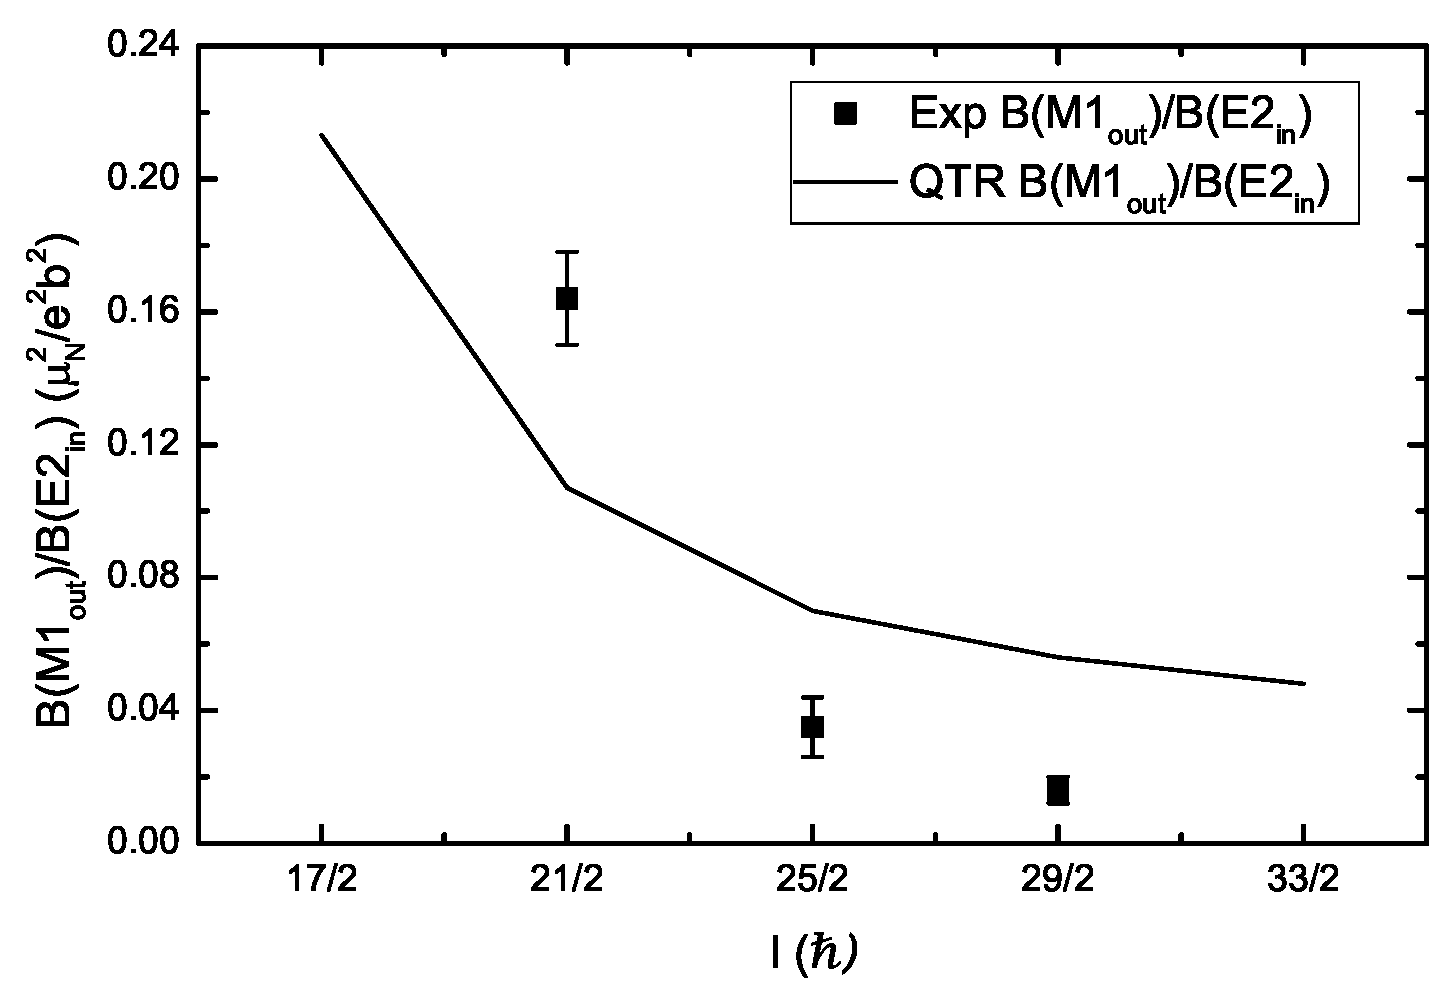
\includegraphics[width=0.455\textwidth]{./img/c4/m1_trans_prob.eps}\hspace{0.08\textwidth}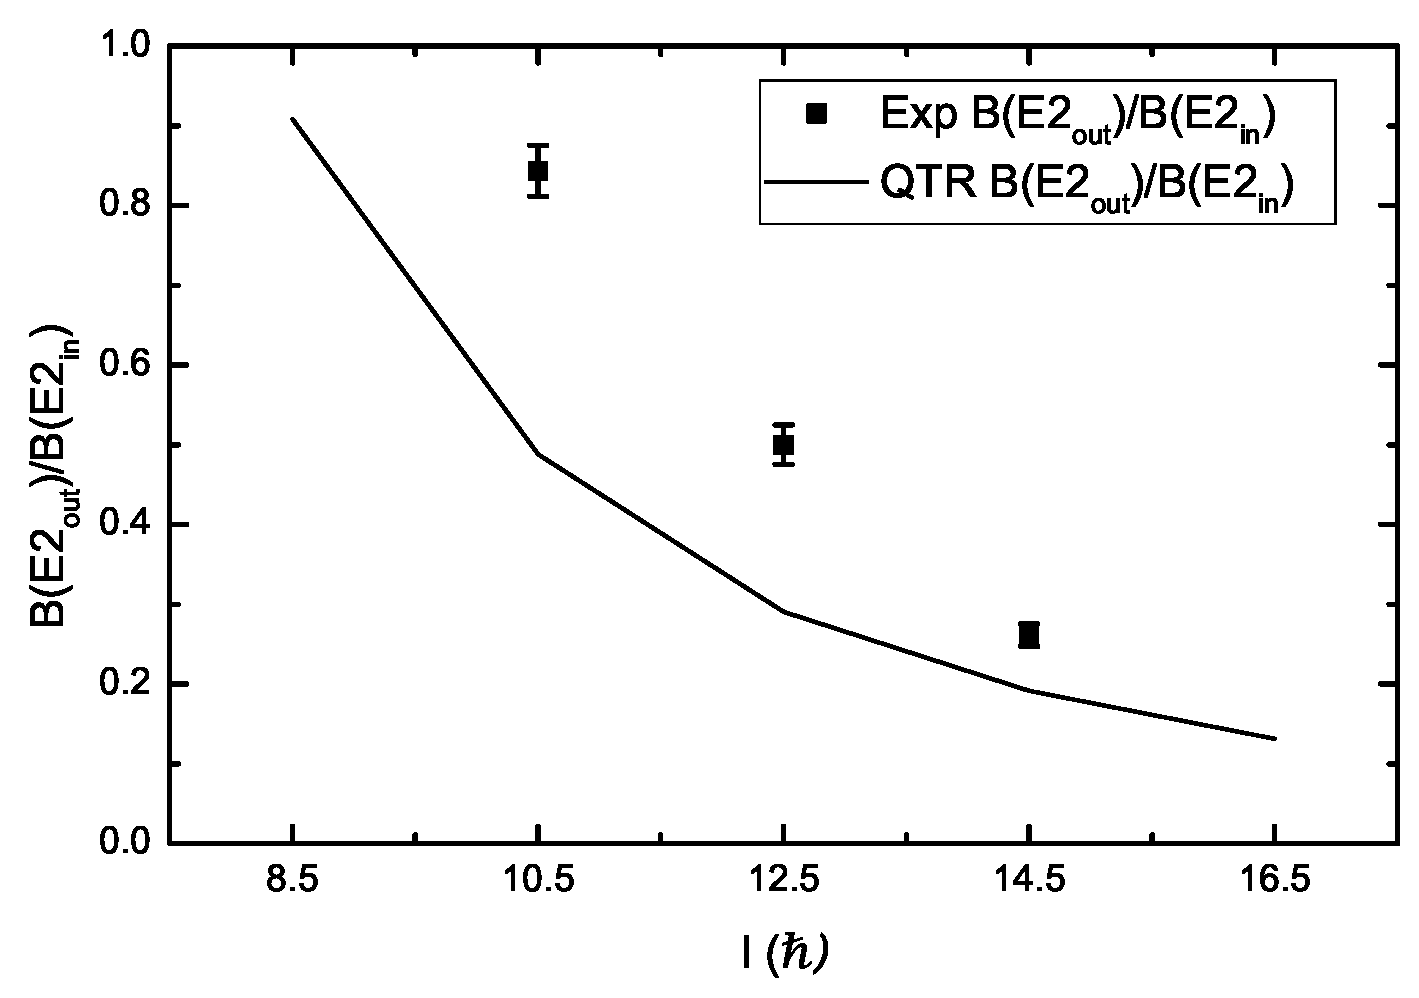
\includegraphics[width=0.45\textwidth]{./img/c4/e2_trans_prob.eps}}
	\caption{Left: Plot of $B(M1_{out})/B(E2_{in})$ ratios for experiment and theory. Right: Plot of $B(E2_{out})/B(E2_{in})$ ratios for experiment and theory.\label{fig:chp4-trans-prob-ratios}}
\end{figure}

TAC calculations were carried out for the one quasiparticle $\pi(h_{11/2}$ yrast band, the five quasiparticle $\pi(h_{11/2}^3\nu(h_{11/2}^2$ yrast band, and the three quasiparticle $\pi(h_{11/2}\nu(h_{11/2}^2$ dipole band 1. For the one quasiparticle yrast band pair gaps of $\Delta_p=1.1$ MeV and $\Delta_n=1.0$ MeV were used and the equilibrium deformation parameters obtained were $\epsilon=0.16$ and $\gamma=26^{\circ}$. For the one quasiparticle yrast band pair gaps of $\Delta_p=0$ MeV and $\Delta_n=0.8$ MeV were used and the equilibrium deformation parameters obtained were $\epsilon=0.20$ and $\gamma=28^{\circ}$. The corresponding MOI of the $\pi(h_{11/2}$ yrast band are then $\mathcal{J}_m,\mathcal{J}_s,\mathcal{J}_l = 19, 8, 3 \hbar{}/MeV$. A QTR calculation using these MOI leads to the early collapse of the wobbling band, this is avoided using the fitted MOI for the QTR model. A plot of the energy levels calculated through the TAC model and those from experiment is in Fig. \ref{fig:chp4-TAC-en}.

\begin{figure}[t!]
\centerline{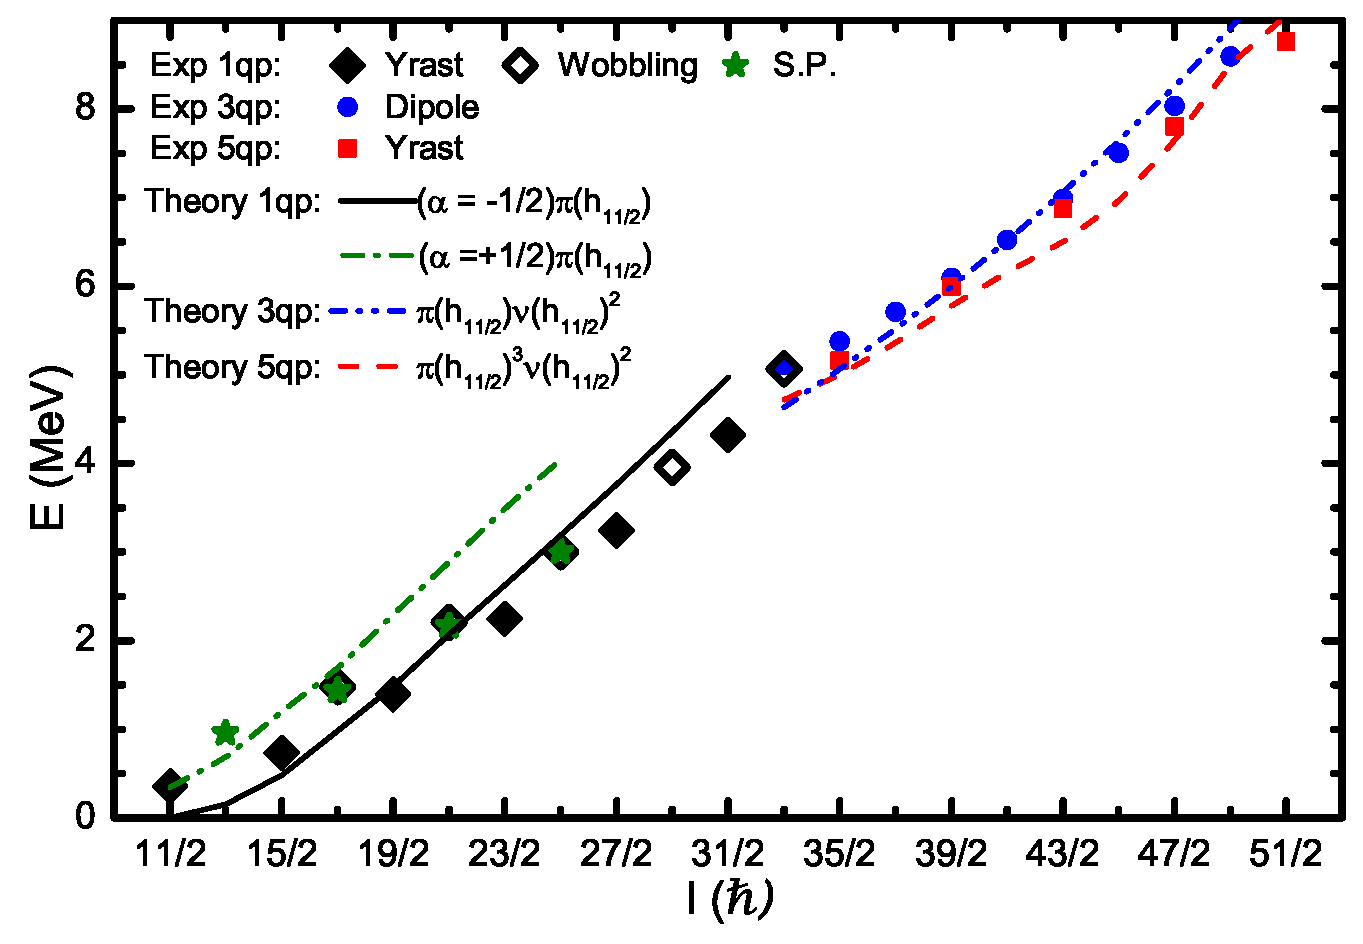
\includegraphics[width=\textwidth]{./img/c4/evj_new_yrast.eps}}
	\caption{Experimental and theoretical level energies for the yrast band, $n_w=1$ band, the signature partner band, and dipole band 1. \label{fig:chp4-TAC-en}}
\end{figure}

\section{Discussion}
\label{sec:trw-discussion}
TAC and QTR calculations were performed to describe the behavior of the yrast band, $n_w=1$ band, the signature partner band, and dipole band 1 of the nucleus \pr{}. As seen in Table \ref{tbl:chp4-transitition-ratios} and the right panel of Fig. \ref{fig:chp4-trans-prob-ratios}, the QTR model predicts a strong unstretched $E2$ component, dominating the $M1$ part, for $n_w=1\rightarrow{}n_w=0$ transitions. But, the calculations under-predict the $B(E2_{out})$ transition probabilities and somewhat overestimate the $B(M1_{out})$ transition probabilities. Additionally, QTR predicts the signature partner band which exhibits very weak transition probabilities to the yrast band ($B(E2_{out})/B(E2_{in})<0.01$ and $B(E2_{out})/B(M1_{in})<0.02\mu^2_N/e^2b^2$). The experimentally estimated values for the $\sfrac{17}{2}^-\rightarrow\sfrac{15}{2}^-$ transition, 0.0002 and 0.004 (respectively), confirm this. The QTR calculations predict the signature partner band to be $\sim{}0.5$ MeV higher than it is found experimentally. The TAC calculations however predict its energy approximately correctly.

With the observation of $\Delta{}I=1, E2$ $n_w=1\rightarrow{}n_w=0$ transitions, transverse wobbling has been show conclusively to exist in \pr{}. The very good agreement between experiment and theoretical models proves the understanding of the phenomenon is robust. Transverse wobbling seems to be the solution to the previous discrepancy between the QTR model wobbling energies \cite{oldQTRWobblingTheory1,oldQTRWobblingTheory2,oldQTRWobblingTheory3,oldQTRWobblingTheory4} and the experimentally observed energies. The previous wobblers $^{161,163,165,167}$Lu \cite{wobblingIn163Lu,wobblingIn163LuTwoPhonon,wobblingIn165Lu,wobblingIn167Lu,wobblingIn161Lu} and $^{167}$Ta \cite{wobblingIn167Ta} should be reevaluated from the perspective of transverse wobbling. Additionally, the discovery of transverse wobbling in \pr{} opens up the $A\sim{}130$ region for a systematic search for other wobbling bands. Finally, the possible $n_w=2$ band gives hope that the wobbling mode in \pr{} is robust enough to support multiple phonons. With a two phonon band in this energy and spin range lifetime measurements could be carried out to examine the wobbling phonon and its nature in detail.